\documentclass[        
    a4paper,          % Tamanho da folha A4
    12pt,             % Tamanho da fonte 12pt
    chapter=TITLE,    % Todos os capitulos devem ter caixa alta
    %section=TITLE,   % Todas as secoes devem ter caixa alta
    oneside,          % Usada para impressao em apenas uma face do papel
    english,          % Hifenizacoes em ingles
    spanish,          % Hifenizacoes em espanhol
    brazil            % Ultimo idioma eh o idioma padrao do documento
]{abntex2}
%%%%%%%%%%%%%%%%%%%%%%%%%%%%%%%%%%%%%%%%%%%%%%%%%%%%%%%%%%%%%%%%%%%%%%%%%%%%%%%
%%% 				Customizações do abnTeX2 para o IFCE    			    %%%
%%% 		Instituto Federal de Educação, Ciência e Tecnologia do Ceará    %%%
%%% Template disponível em: https://github.com/clodomirneto/IFCETeX2	    %%%
%%% Desenvolvedores do IFCETeX2: Professor Clodomir Silva Lima Neto		    %%%
%%% 							 Professor Marcelo Araújo Lima              %%%
%%%                              Professor Antonio Sergio de Sousa Vieira	%%%
%%% E-mails para contato: clodomir.neto@ifce.edu.br						    %%%
%%% 					  marcelo.alima@ifce.edu.br                         %%%
%%%                       sergio.vieira@ifce.edu.br	                        %%%
%%%%%%%%%%%%%%%%%%%%%%%%%%%%%%%%%%%%%%%%%%%%%%%%%%%%%%%%%%%%%%%%%%%%%%%%%%%%%%%

% Importações de pacotes
\usepackage[utf8]{inputenc}                         % Acentuação direta
\usepackage[T1]{fontenc}                            % Codificação da fonte em 8 bits
\usepackage{graphicx}                               % Inserir figuras
\usepackage{calc}
\usepackage{svg}
\usepackage{amsfonts,amssymb,amsmath}               % Fonte e símbolos matemáticos
\usepackage{mathtools}
\usepackage{cancel}
\usepackage{booktabs}                               % Comandos para tabelas
\usepackage{verbatim}                               % Texto é interpretado como escrito no documento
\usepackage{multirow,array}                         % Múltiplas linhas e colunas em tabelas
\usepackage{indentfirst}                            % Endenta o primeiro parágrafo de cada seção.
\usepackage{listings}                               % Utilizar codigo fonte no documento
\usepackage{xcolor}
\usepackage{microtype}                              % Para melhorias de justificação?
\usepackage[portuguese,ruled,lined]{algorithm2e}    % Escrever algoritmos
% \usepackage{algorithm}
% \usepackage{algpseudocode}
% \usepackage{algorithmic}                            % Criar Algoritmos  
%\usepackage{float}                                 % Utilizado para criação de floats
\usepackage{amsgen}
\usepackage{lipsum}                                 % Usar a simulação de texto Lorem Ipsum
%\usepackage{titlesec}                               % Permite alterar os títulos do documento
\usepackage{tocloft}                                % Permite alterar a formatação do Sumário
\usepackage{etoolbox}                               % Usado para alterar a fonte da Section no Sumário
%\usepackage[nogroupskip,nonumberlist,acronym]{glossaries}                % Permite fazer o glossario
\usepackage{caption}                                % Altera o comportamento da tag caption
\usepackage[alf,abnt-emphasize=bf,bibjustif, recuo=0cm,abnt-etal-cite=3,abnt-etal-list=0,abnt-etal-text=it]{abntex2cite}  % Citações padrão ABNT
%\usepackage[bottom]{footmisc}                      % Mantém as notas de rodapé sempre na mesma posição
%\usepackage{times}                                 % Usa a fonte Times
\usepackage{mathptmx}                               % Usa a fonte Times New Roman							
\usepackage{lmodern}                               % Usa a fonte Latin Modern
%\usepackage{subfig}                                % Posicionamento de figuras
%\usepackage{scalefnt}                              % Permite redimensionar tamanho da fonte
%\usepackage{color, colortbl}                       % Comandos de cores
\usepackage{lscape}                                 % Permite páginas em modo "paisagem"
\usepackage{pdflscape}
%\usepackage{ae, aecompl}                           % Fontes de alta qualidade
%\usepackage{picinpar}                              % Dispor imagens em parágrafos
%\usepackage{latexsym}                              % Símbolos matemáticos
%\usepackage{upgreek}                               % Fonte letras gregas
\usepackage{appendix}                               % Gerar o apendice no final do documento
\usepackage{paracol}                                % Criar paragrafos sem identacao
\usepackage{ifcetex2}		                        % Biblioteca com as normas do IFCE para trabalhos academicos
\usepackage{pdfpages}                               % Incluir pdf no documento
\usepackage{textcomp}
\usepackage{listings}
\usepackage{courier}
\usepackage{float}
\usepackage{makecell}
% Organiza e gera a lista de abreviaturas, simbolos e glossario
%\makeglossaries
% Gera o Indice do documento
%\makeindex

%TEOREMAS

\newtheorem{proposition}{Proposição}[chapter]
\newtheorem{theorem}{Teorema}[chapter]
\newtheorem{lemma}{Lema}[chapter]
\newtheorem{definition}{Definição}[chapter]
\newtheorem{exemplo}{Exemplo}[chapter]
\newtheorem{corollary}{Corolário}[chapter]
\newtheorem{exercicio}{Exercício}[chapter]

%PROVAS

\newenvironment{prova}[1][Prova]{\noindent\textbf{#1.} }{\hfill\rule{0.5em}{0.5em}}
\newenvironment{dem}[1][Demonstra\c c\~ao]{\noindent\textbf{#1.} }{\hfill\rule{0.5em}{0.5em}}
\newenvironment{exm}{\noindent{\textbf{Exemplo:}}}{}

% Alg
% \SetKwRepeat{Repita}{repita}{enquanto}

\renewcommand{\arraystretch}{1.5}
\setlength{\tabcolsep}{12pt}

\renewcommand{\lstlistlistingname}{Lista de algoritmos}
\renewcommand{\lstlistingname}{Algoritmo}

\definecolor{back}{rgb}{0.,0.,0.}
\definecolor{codegreen}{rgb}{0,0.6,0}
\definecolor{codegray}{rgb}{0.5,0.5,0.5}
\definecolor{codepurple}{rgb}{0.58,0,0.82}
\definecolor{backcolour}{rgb}{0.95,0.95,0.92}
\definecolor{backcolorgray}{rgb}{0.95703125,0.95703125,0.95703125}

\lstdefinestyle{mystyle}{
    % backgroundcolor=\color{backcolorgray},
    commentstyle=\color{codegray},
    % keywordstyle=\color{back},
    keywordstyle=\bfseries,
    % numberstyle=\tiny\color{codegray},
    % stringstyle=\color{codepurple},
    basicstyle=\ttfamily\footnotesize,
    % breakatwhitespace=false,
    breaklines=true,
    % captionpos=b,
    % keepspaces=true,
    numbers=left,
    % numbersep=5pt,
    % showspaces=false,
    % showstringspaces=false,
    % showtabs=false,
    % tabsize=2
    frame=none,
    % xleftmargin=10pt
    framexleftmargin=2pt,
    % framexleftmargin=10pt
}

\lstset{style=mystyle}

\lstset{literate=
  {á}{{\'a}}1 {é}{{\'e}}1 {í}{{\'i}}1 {ó}{{\'o}}1 {ú}{{\'u}}1
  {Á}{{\'A}}1 {É}{{\'E}}1 {Í}{{\'I}}1 {Ó}{{\'O}}1 {Ú}{{\'U}}1
  {ã}{{\~a}}1 {õ}{{\~o}}1 {ç}{{\c{c}}}1 {Ç}{{\c{C}}}1
}

% \lstset{basicstyle=\footnotesize\ttfamily,breaklines=true}
% \lstset{framextopmargin=50pt,frame=shadowbox}
% \lstset{framextopmargin=50pt,frame=bottomline}

\let\oldlstlistoflistings\lstlistoflistings
\renewcommand{\lstlistoflistings}{%
  \begingroup
  \let\oldaddcontentsline\addcontentsline % Save the original \addcontentsline
  \renewcommand{\addcontentsline}[3]{} % Redefine \addcontentsline to do nothing
  \oldlstlistoflistings % Call the original \lstlistoflistings
  \endgroup
}
\newcommand{\imprimirlistadecodigos}{
	\lstlistoflistings
	\pagebreak %
}

\newenvironment{courierfont}{\fontfamily{pcr}\selectfont}{\par}

% Forest

\usepackage[edges]{forest}

\definecolor{foldercolor}{RGB}{124,166,198}

\tikzset{pics/folder/.style={code={%
    \node[inner sep=0pt, minimum size=#1](-foldericon){};
    \node[folder style, inner sep=0pt, minimum width=0.3*#1, minimum height=0.6*#1, above right, xshift=0.05*#1] at (-foldericon.west){};
    \node[folder style, inner sep=0pt, minimum size=#1] at (-foldericon.center){};}
    },
    pics/folder/.default={20pt},
    folder style/.style={draw=foldercolor!80!black,top color=foldercolor!40,bottom color=foldercolor}
}

\forestset{is file/.style={edge path'/.expanded={%
        ([xshift=\forestregister{folder indent}]!u.parent anchor) |- (.child anchor)},
        inner sep=1pt},
    this folder size/.style={edge path'/.expanded={%
        ([xshift=\forestregister{folder indent}]!u.parent anchor) |- (.child anchor) pic[solid]{folder=#1}}, inner xsep=0.7*#1},
    folder tree indent/.style={before computing xy={l=#1}},
    folder icons/.style={folder, this folder size=#1, folder tree indent=3*#1},
    folder icons/.default={12pt},
}

% resize sum [https://tex.stackexchange.com/a/81711]
\newlength{\depthofsumsign}
\setlength{\depthofsumsign}{\depthof{$\sum$}}
\newlength{\totalheightofsumsign}
\newlength{\heightanddepthofargument}

\newcommand{\nsum}[1][1.4]{% only for \displaystyle
    \mathop{%
        \raisebox
            {-#1\depthofsumsign+1\depthofsumsign}
            {\scalebox
                {#1}
                {$\displaystyle\sum$}%
            }
    }
}
\newcommand{\resum}[1]{%
    \def\s{#1}
    \mathop{
        \mathpalette\resumaux{#1}
    }
}

\newcommand{\resumaux}[2]{% internally
    \sbox0{$#1#2$}
    \sbox1{$#1\sum$}
    \setlength{\heightanddepthofargument}{\wd0+\dp0}
    \setlength{\totalheightofsumsign}{\wd1+\dp1}
    \def\quot{\DivideLengths{\heightanddepthofargument}{\totalheightofsumsign}}
    \nsum[\quot]%
}

% http://tex.stackexchange.com/a/6424/16595
\makeatletter
\newcommand*{\DivideLengths}[2]{%
  \strip@pt\dimexpr\number\numexpr\number\dimexpr#1\relax*65536/\number\dimexpr#2\relax\relax sp\relax
}
\makeatother

% Big O notation
\newcommand\bigO[1]{$\mathcal{O}(#1)$}


\trabalhoacademico{tccgraduacao}

% Define se o trabalho é uma qualificação, coloque 'nao' para versão final do trabalho
\ehqualificacao{nao}

% Remove as bordas vermelhas e verdes do PDF gerado, coloque 'sim' para remover
\removerbordasdohyperlink{sim} 

% Adiciona a cor azul a todos os hyperlinks
\cordohyperlink{nao}

% Informação relacionadas ao trabalho
\autor{João Breno Rodrigues Venancio}
\titulo{O problema de ordenação: algoritmos}
\local{Fortaleza}
\data{2024}

% Informação sobre a IES
\ies{Instituto Federal de Educação, Ciência e Tecnologia do Ceará}
\iessigla{IFCE}
\centro{\textit{Campus} Fortaleza}

% Informação para TCC de Graduação
\graduacaoem{Bacharelado em Engenharia da Computação} 
\habilitacao{Bacharel} % Licenciado ou Bacharel
\areadeconcentracaograduacao{Engenharia da Computação}

% Data de Aprovação
\dataaprovacao{\underline{\hspace*{1cm}}/\underline{\hspace*{1cm}}/\underline{\hspace*{1.2cm}}.}

% Abreviaturas dos títulos acadêmicos

% Especialista: Esp.
% Mestre: Me.
% Mestra: Ma.
% Doutor: Dr.
% Doutora: Dra.

% Informação sobre o Orientador
\orientador{Prof. Dr. Glauber Ferreira Cintra}
\orientadories{Instituto Federal de Educação, Ciência e Tecnologia do Ceará}
\orientadoriessigla{IFCE}
\orientadorcentro{\textit{Campus} Fortaleza}
\orientadorfeminino{nao} % Coloque 'sim' se for do sexo feminino

% Informação sobre o Coorientador
\coorientador{} % Deixe o nome do coorientador em branco para remover do documento
\coorientadories{Instituto Federal de Educação, Ciência e Tecnologia do Ceará}
\coorientadoriessigla{IFCE}
\coorientadorcentro{\textit{Campus} Caucaia}
\coorientadorfeminino{sim} % Coloque 'sim' se for do sexo feminino

% Informação sobre a banca
% Membro da Banca Dois
\membrodabancadois{Prof. Dra. XXXXX}
\membrodabancadoisies{Instituto Federal de Educação, Ciência e Tecnologia do Ceará}
\membrodabancadoisiessigla{IFCE}
\membrodabancadoiscentro{\textit{Campus} Caucaia}

% Membro da Banca Três
\membrodabancatres{Prof. Dra. XXXXX}
\membrodabancatresies{Instituto Federal de Educação, Ciência e Tecnologia do Ceará}
\membrodabancatresiessigla{IFCE}
\membrodabancatrescentro{\textit{Campus} Caucaia}

% Informação Complementar sobre a banca
\membrodabancaquatro{Membro da Banca Quatro}
\membrodabancaquatrocentro{Centro de Ciências e Tecnologia - CCT}
\membrodabancaquatroies{Universidade do Membro da Banca Quatro - SIGLA}
\membrodabancacinco{Membro da Banca Cinco}
\membrodabancacincocentro{Teste}
\membrodabancacincoies{Universidade do Membro da Banca Cinco - SIGLA}
\membrodabancaseis{Membro da Banca Seis}
\membrodabancaseiscentro{}
\membrodabancaseisies{Universidade do Membro da Banca Seis - SIGLA}

\begin{document}	

% Elementos pré-textuais
% \imprimircapa
% \imprimirfolhaderosto{}
% \imprimirfichacatalografica{elementos-pre-textuais/ficha-catalografica}
% \imprimirfolhadeaprovacao
% \imprimirdedicatoria{elementos-pre-textuais/dedicatoria}
% \imprimiragradecimentos{elementos-pre-textuais/agradecimentos}
% \imprimirepigrafe{elementos-pre-textuais/epigrafe}
% \imprimirresumo{elementos-pre-textuais/resumo}
% \imprimirabstract{elementos-pre-textuais/abstract}
% \imprimirlistadefiguras
% \imprimirlistadetabelas
% \imprimirlistadesiglas{elementos-pre-textuais/lista-de-siglas}
% \imprimirlistadesimbolos{elementos-pre-textuais/lista-de-simbolos}
\imprimirsumario

% Elementos textuais
\textual
\chapter{Introdução}\label{cap:introducao}
Este trabalho está dividido em $7$ capítulos. Neste primeiro capítulo introdutório, serão definidos o problema da ordenação e sua importância. No capítulo seguinte, serão apresentados alguns dos conceitos que serão importantes para o entendimento do conteúdo que se segue. Os próximos três capítulos ($3$, $4$ e $5$) apresentarão, ao todo, $14$ algoritmos que resolvem o problema da ordenação, bem como suas implementações, complexidades temporais e espaciais, dentre outras características. O capítulo $6$ realizará, então, uma análise empírica a partir dos resultados obtidos com a execução dos algoritmos, à luz de determinadas métricas. Por fim, o último capítulo trará uma conclusão.

\section{O problema da ordenação}
O problema da ordenação consiste em reorganizar uma sequência de dados para que seus elementos estejam dispostos em uma ordem específica, geralmente crescente ou decrescente. Em termos formais, o problema pode ser definido da seguinte maneira: dada uma sequência de  $n$  números  $\langle a_1, a_2, ..., a_n \rangle$, produzir uma permutação $\langle a_1', a_2', ..., a_n' \rangle$ da sequência de entrada, tal que $a_1' \le a_2' \le ... \le a_n'$  \cite[p. 5]{Cormen2009}.

A ordenação é uma das operações fundamentais em computação, com aplicações diretas em diversas áreas, como pesquisa, organização de dados, algoritmos de busca e análise estatística. Além disso, é uma etapa essencial em muitos outros algoritmos, como aqueles utilizados em análise de grafos, aprendizado de máquina e simulação de sistemas.

A importância do problema da ordenação também está relacionada à sua presença em problemas cotidianos, como organização de listas de compras, ordenação de arquivos em sistemas operacionais, ordenação de registros em bancos de dados e priorização de tarefas em filas de execução. Além disso, a resolução desse problema proporciona uma base teórica para o estudo de outros problemas mais complexos em computação.

Compreender e resolver eficientemente o problema da ordenação é crucial para otimizar o desempenho de sistemas computacionais. A escolha de um algoritmo adequado para um determinado cenário pode impactar significativamente os requisitos de tempo e espaço, especialmente em aplicações que envolvem grandes volumes de dados. Assim, o estudo da ordenação não só permite avanços na própria área de computação, mas também contribui para soluções mais eficientes em diversas áreas do conhecimento.

\chapter{Preliminares}\label{cap:preliminares}
\section{Ordenação interna e externa}
A ordenação pode ser classificada em dois tipos principais: interna e externa, dependendo da forma como os dados são manipulados durante o processo de ordenação.

Ordenação interna ocorre quando todos os dados a serem ordenados cabem na memória principal do computador (RAM). Esse tipo de ordenação é amplamente utilizado em cenários onde o volume de dados é relativamente pequeno e o acesso rápido à memória permite um desempenho eficiente.

Ordenação externa, por outro lado, é aplicada quando o volume de dados é tão grande que excede a capacidade da memória principal, necessitando do uso de memória secundária, como discos rígidos ou SSDs. Nesse caso, os algoritmos devem ser projetados para minimizar o número de acessos à memória secundária, que é consideravelmente mais lenta do que a memória principal. Exemplos incluem algoritmos de ordenação por blocos e Mergesort externo.

Neste trabalho, o foco será exclusivamente na ordenação interna, abordando os principais algoritmos utilizados, suas características e desempenhos em diferentes cenários.

\section{Ordenação estável}
A ordenação é considerada estável quando preserva a ordem relativa dos elementos com chaves iguais na sequência de entrada. Em outras palavras, se dois elementos possuem a mesma chave e um deles aparece antes do outro na sequência original, um algoritmo de ordenação estável garantirá que essa ordem relativa seja mantida na sequência ordenada.

A estabilidade em algoritmos de ordenação é especialmente importante em cenários onde os elementos possuem atributos adicionais além da chave utilizada para a ordenação. Por exemplo, em um sistema de gerenciamento de registros, onde cada registro é identificado por um nome e uma data, a estabilidade permite ordenar os registros primeiro por nome e, em seguida, por data, sem perder a ordem relativa estabelecida na primeira ordenação.

A Tabela \ref{tab:estabilidade} apresenta os algoritmos que serão implementados neste trabalho e indica quais deles são estáveis:

\begin{table}[!h]
    \centering
    \Caption{\label{tab:estabilidade}Estabilidade dos algoritmos apresentados}
    \begin{tabular}{ | c | l |  }
    \hline
    Algoritmo    & Estável    \\
    \hline
    Bolha        & \checkmark \\
    Coquetel     & \checkmark \\
    Selecao      &            \\
    Insercao     & \checkmark \\
    Shellsort    &            \\
    Mergesort    & \checkmark \\
    Heapsort     &            \\
    Quicksort    &            \\
    Countingsort & \checkmark \\
    Bucketsort   & \checkmark \\
    RadixsortC   & \checkmark \\
    RadixsortB   & \checkmark \\
    \hline
    \end{tabular}
\end{table}


\section{Análise de algoritmos}

\subsection{Notação assintótica}
A Notação Assintótica é um conjunto de ferramentas matemáticas utilizada na análise de algoritmos para descrever o comportamento limitante ou de crescimento de uma função à medida que o tamanho da entrada se aproxima do infinito. Seu propósito principal é fornecer uma forma de classificar e comparar a eficiência de algoritmos, focando apenas na ordem de magnitude do tempo ou espaço consumido e ignorando constantes de proporcionalidade e termos de ordem inferior. Ao expressar a complexidade de tempo de um algoritmo, a notação assintótica permite prever como o algoritmo escalará em grandes volumes de dados, independentemente de detalhes de implementação ou da velocidade específica do hardware.

Definir a complexidade de um algoritmo exige o uso de notações assintóticas precisas para delimitar seu comportamento. A notação \bigO{f(n)} fornece um limite superior para complexidade de um algoritmo, seja ela temporal ou espacial, descrevendo o pior caso. Ela significa que, para valores grandes de entrada $n$, a complexidade nunca será pior do que uma função $c \cdot f(n)$, onde $c$ é uma constante positiva e $f(n)$ é a função de crescimento. Já a notação $\Theta(f(n))$ fornece um limite assintótico apertado, definindo o comportamento exato da complexidade de um algoritmo. Isso significa que, para $n$ grande, a complexidade está limitado superior e inferiormente por múltiplos constantes de $f(n)$, indicando que $f(n)$ é a ordem de crescimento precisa, tanto no melhor quanto no pior caso.

\subsection{Cota inferior}\label{subsec:cota-inferior}
Cota inferior define o limite mínimo de desempenho necessário para resolver um problema. Isso significa que nenhum algoritmo pode resolver o problema em menos tempo do que a cota inferior definida, independentemente da abordagem utilizada. A notação usada para descrever a cota inferior é a notação $\Omega(f(n))$.

Para algoritmos de ordenação baseados em comparação, a cota inferior é $\Omega(n\log_2n)$. Esse resultado demonstra que qualquer algoritmo de ordenação que utilize apenas comparações entre elementos, no pior caso, precisará de pelo menos $n\log_2n$ comparações para ordenar n elementos. Este limite foi provado por \cite{knuth1998art}, onde ele utiliza conceitos de árvores de decisão para demonstrar que a profundidade mínima da árvore que representa todas as permutações possíveis dos elementos é $\log_2(n!)$, o que se aproxima de $n\log_2n$ pela fórmula de Stirling.

\subsection{Divisão e conquista e Teorema mestre}
O paradigma Divisão e conquista é uma das estratégias mais poderosas no projeto de algoritmos, na qual um problema complexo é resolvido de forma recursiva por meio de três etapas: dividir, conquistar e combinar. Na etapa de divisão, o problema original de tamanho $n$ é quebrado em $a$ subproblemas menores, cada um de tamanho $n/b$. Na etapa de conquista, os subproblemas são resolvidos recursivamente. Finalmente, na etapa de combinação, as soluções dos subproblemas são reunidas para formar a solução final do problema original.

A eficiência de um algoritmo que segue o paradigma Divisão e conquista é caracterizada por uma relação de recorrência da forma $T(n) = aT(n/b) + f(n)$, sendo que $T(n)$ representa o tempo total de execução. O Teorema Mestre é a ferramenta matemática que permite solucionar essas recorrências e determinar sua complexidade assintótica. Ele funciona comparando o custo do trabalho de divisão e combinação, $f(n)$, com o custo do trabalho realizado nas folhas da árvore de recursão, dado por $n^{\log_b a}$. O teorema afirma que a solução $T(n)$ cairá em um de três casos:
\begin{itemize}
    \item Se $f(n)$ for assintoticamente menor que $n^{\log_b a}$, a complexidade será $O(n^{\log_b a})$;
    \item Se $f(n)$ for assintoticamente maior, a complexidade será $O(f(n))$;
    \item E se forem assintoticamente iguais, a complexidade será $O(n^{\log_b a} \log n)$.
\end{itemize}  

\subsection{Probabilidade e valor esperado}
A probabilidade é a medida numérica da chance de um evento específico ocorrer, variando de zero (impossibilidade) a um (certeza), e é fundamental para modelar a incerteza. Já o valor esperado (ou esperança matemática) é uma medida que resume o resultado mais provável ou a média de longo prazo de um fenômeno aleatório. Ele é calculado ponderando-se cada resultado possível pelo seu respectivo valor de probabilidade, oferecendo uma estimativa útil para a tomada de decisões em cenários de risco, como jogos de azar ou análises financeiras.

Esses dois conceitos matemáticos serão utilizados no próximo capítulo para a análise de complexidade da versão probabilística do algoritmo Quicksort.

\section{Arquitetura de computadores}\label{sec:arquitetura}
A análise de complexidade \bigO{f(n)} é fundamental, mas não é o único fator que determina o tempo de execução real. Em sistemas de computação modernos, a hierarquia de memória e o conceito de localidade de referência também ajudam a entender o desempenho.

\subsection{Hierarquia de memória}
O processador (CPU) interage com diferentes níveis de memória que variam drasticamente em velocidade de acesso e capacidade de armazenamento. A Tabela \ref{tab:memory-hierarchy}, apresentada a seguir, relaciona os tipos de memória com suas capacidades e velocidades. Como os valores exatos de capacidade e latência podem variar entre fabricantes e modelos, esta é uma classificação em alto nível que se mantém consistente, independentemente desses fatores.

\begin{table}[!h]
    \centering
    \Caption{\label{tab:memory-hierarchy}Capacidade e velocidade de acesso por tipo de memória}
    \begin{tabular}{ | c | l | l |  }
    \hline
    Nível de memória             & Capacidade  & Velocidade de acesso\\
    \hline
    Registradores/L1 Cache       & Muito Baixa & Extremamente rápido \\
    L2/L3 Cache                  & Baixa       & Muito rápido        \\
    Memória principal (RAM)      & Alta        & Lento               \\
    Memória secundária (SSD/HDD) & Muito Alta  & Muito lento         \\
    \hline
    \end{tabular}
\end{table}

O processador é muito rápido. Uma operação básica, como uma comparação ou soma, pode levar apenas um ciclo de clock. No entanto, quando ocorre uma falha de cache — isto é, quando se busca por um dado que não está no cache e precisa ser carregado da RAM — o processo pode custar dezenas ou até centenas de ciclos de clock. Desse modo, a velocidade de um algoritmo em um grande conjunto de dados é frequentemente limitada pelo tempo gasto esperando o acesso à memória, e não pelo número de operações da CPU


\subsection{Localidade de referência}\label{subsec:localidade-referencia}
Para mitigar o alto custo de acesso à RAM, os processadores utilizam um princípio chamado localidade de referência. Este princípio se refere à tendência de um programa de acessar o mesmo conjunto de locais de memória ou locais próximos em um curto período de tempo.

\begin{itemize}
    \item Localidade temporal: Se um item foi acessado, é provável que ele seja acessado novamente em breve.
    \item Localidade espacial: Se um item foi acessado, é provável que os itens armazenados em endereços de memória próximos sejam acessados em breve.
\end{itemize}

A eficiência de cache é aumentada porque o cache opera em ``blocos'' ou ``linhas de cache'', geralmente de 64 bytes. Ou seja, quando um dado $v[i]$ não está no cache e a CPU precisa carregá-lo da RAM, ela não carrega apenas $v[i]$, mas sim um bloco inteiro que contém $v[i]$ e vários elementos adjacentes, como $v[i+1]$, $v[i+2]$, etc.

Se um algoritmo seguir a localidade espacial, acessando sequencialmente $v[i]$, $v[i+1]$, $v[i+2]$, ele encontrará os próximos dados que precisa já carregados no cache. Assim, o custo de esperar a RAM é pago apenas uma vez para o bloco inteiro, o que torna o acesso subsequente, linear e sequencial quase instantâneo.

Algoritmos que varrem grandes vetores de forma sequencial maximizam a Localidade Espacial e, por isso, são considerados ``cache-friendly''. Em contraste, algoritmos que ``pulam'' em endereços de memória dispersos desperdiçam o bloco de cache carregado e incorrem em muitas falhas de cache.

\chapter{Métodos inferiores}\label{cap:inferiores}
Neste capítulo, são apresentados quatro algoritmos básicos para o problema da ordenação. Esses algoritmos são chamados de inferiores por serem simples, intuitivos e, principalmente, por apresentarem, no mínimo, complexidade temporal quadrática nos casos médio e pior.

\section{Bolha}
O algoritmo Bolha é um dos algoritmos mais simples para o problema da ordenação. Ele consistem em percorrer várias vezes o vetor, comparando elementos adjacentes e trocando-os de posição caso estejam fora da ordem desejada. Nesse processo, os elementos flutuam para suas posições finais. Em outras palavras, ``[...]  os elementos da lista são movidos para as posições adequadas de forma contínua, assim como uma bolha move-se num líquido. Se um elemento está inicialmente numa posição i e, para que a lista fique ordenada, ele deve ocupar a posição j, então ele terá que passar por todas as posições entre i e j.'' \cite[p.8]{viana2011pesquisa}.

\lstinputlisting[language=C]{codigos/inf/1_bolha.txt}

Esta versão do algoritmo Bolha é também conhecida como ``Bolha com Flag'', por conta do uso da variável \textit{trocou}. Perceba que, sem essa variável, o algoritmo continua funcionando da mesma forma; porém o laço externo executará sempre $n - 1$ iterações, mesmo que o vetor fique ordenado antes.

Observe que o algoritmo Bolha oferece uma ordenação estável, pois, quando dois elementos adjacentes são iguais, eles não são trocados.

\subsection*{Corretude}
Ao final de uma iteração do laço externo, o maior elemento de $v[0..i]$ estará na posição $i$. Dessa forma, ao final da primeira iteração, o maior elemento do vetor estará na posição $n - 1$; ao final da segunda iteração, o segundo maior estará na posição $n - 2$, e assim por diante. Portanto, o algoritmo Bolha é correto.

\subsection*{Desempenho}
Em termos de consumo de memória adicional, o algoritmo declara apenas três variáveis escalares, sendo duas delas para controle de laço de repetição. Logo, sua complexidade espacial é $\Theta(1)$. Esta observação será omitida para os algoritmos apresentados a seguir que tenham a mesma complexidade espacial.

Já para a complexidade temporal, o melhor caso ocorre quando a entrada já está ordenada em ordem crescente, pois não é realizada nenhuma troca. Exige-se, assim, apenas uma iteração do laço externo, resultando em complexidade $\Theta(n)$.

Por outro lado, o pior caso ocorre quando o menor elemento está na última posição, sendo necessárias exatamente $n - 1$ iterações do laço externo para que ele chegue à primeira posição. Com isso, a quantidade de iterações do laço interno é dada pela seguinte soma:
\begin{equation}\label{eq:1}
    \sum_{i=1}^{n-1} i = \frac{n(n-1)}{2}
\end{equation}
Isso implica em uma complexidade quadrática $\Theta(n^2)$. Em média, a complexidade temporal do algoritmo Bolha é \bigO{n^2}.

\section{Coquetel}
O Coquetel é um algoritmo de ordenação estável que traz a mesma ideia do Bolha, mas com um laço interno adicional. O primeiro laço, assim como no Bolha, itera da esquerda para a direita, empurrando os maiores elementos para o final do vetor, enquanto o segundo itera no outro sentido, empurrando os menores elementos para o início.

\lstinputlisting[language=C]{codigos/inf/2_coquetel.txt}

\subsection*{Corretude}
Ao final de uma iteração do laço externo, o menor e o maior elemento de $v[i..j]$ estarão nas posições $i$ e $j$, respectivamente. Dessa forma, ao final da primeira iteração, o menor elemento estará na posição $0$ e o maior, na posição $n - 1$; na segunda, o segundo menor, na posição $1$, e o segundo maior, na posição $n - 2$, e assim por diante. Esse processo garante que, quando $i \geq j$, o vetor estará ordenado; portanto, o algoritmo é correto.

\subsection*{Desempenho}
Embora as complexidades dos casos melhor, pior e médio continuem sendo, respectivamente, $\Theta(n)$, $\Theta(n^2)$ e \bigO{n^2}, o pior caso do Coquetel é menos frequente, pois ocorre apenas quando a entrada está em ordem decrescente.

\begin{figure}[H]
\Caption{\label{fig:coquetel_it}Coquetel aplicado ao vetor $[n, n-1, ..., 2, 1]$.}
\centering
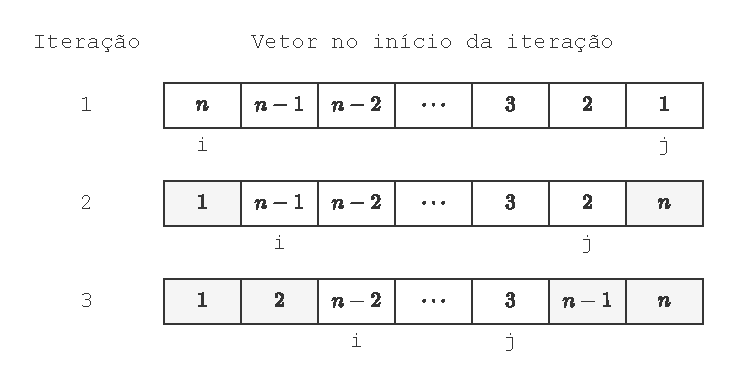
\includegraphics[scale=1.0]{figuras/pdf/coquetel.pdf}
\Fonte{Elaborado pelo autor.}
\end{figure}

Considere então que $T(n)$ é a quantidade total de iterações dos dois laços internos no pior caso. A figura \ref{fig:coquetel_it} ajuda a notar que a seguinte identidade é válida:

\[
T(n) = 
  \begin{cases}
      0,              & n < 2    \\
      T(n-2) + 2n - 3, & n \geq 2 
  \end{cases}
\]

Ao resolver a recorrência mostrada acima, pode-se observar que $T(n)$ é igual a soma \ref{eq:1}. Portanto, os algoritmos Bolha e Coquetel, em seus piores casos, executam exatamente a mesma quantidade de iterações.

\section{Seleção}
O algoritmo Seleção é um método de ordenação instável, como mostra a figura \ref{fig:selecao}. A ideia é bastante simples: execute $n$ iterações; na i-ésima iteração, selecione o i-ésimo menor elemento e coloque-o na posição $i - 1$. Uma propriedade interessante desse algoritmo é que ele realiza o número mínimo possível de trocas para ordenar o vetor.

\lstinputlisting[language=C]{codigos/inf/3_selecao.txt}

\begin{figure}[H]
\Caption{\label{fig:selecao}Seleção aplicado ao vetor \([3, 3, 2, 5]\).}
\centering
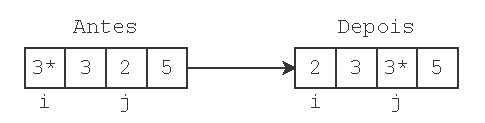
\includegraphics[scale=1.0]{figuras/pdf/selecao.pdf}
\Fonte{Elaborado pelo autor}
\end{figure}

\subsection*{Corretude}
É invariante que, ao final de cada iteração do laço externo, os elementos de $v[0..i]$ já estejam em suas posições definitivas. Portanto, ao final da última iteração, quando $i$ for igual a $n - 1$, o vetor $v[0..n - 1]$ estará ordenado.

\subsection*{Desempenho}
O ponto crítico do algoritmo Seleção é o teste condicional \textit{if} na linha 5. A quantidade de vezes que esse ponto é executado é sempre dada pela soma \ref{eq:1}, ou seja, não há melhor nem pior caso. Portanto, esse algoritmo sempre requer tempo igual a $\Theta(n^2)$.

\section{Inserção}
O algoritmo Inserção é um método de ordenação estável com o melhor desempenho entre os métodos inferiores. A ideia por trás do algoritmo é simples: para $i$ variando de $1$ a $n - 1$, nesta ordem, insira $v[i]$ em $v[0..i - 1]$, de modo que $v[0..i]$ esteja em ordem.

Em especial, o algoritmo Inserção possui complexidade temporal linear para entradas quase ordenadas. Por conta disso, outros algoritmos fazem uso dele como sub-rotina. O Shellsort, por exemplo, utiliza o Inserção para tornar o vetor $h$-ordenado.

\begin{definition}
Para um dado número natural $h > 0$, um vetor $v$ de tamanho $n$ é considerado $h$-ordenado quando $v[i] \leq v[i + h]$, para todo $0 \leq i < n - h$.
\end{definition}

\lstinputlisting[language=C]{codigos/aux/h-ordena.txt}

A implementação do Inserção pode ser idêntica à função H\_Ordena mostrada acima, bastando fazer $h = 1$, pois, nesse caso em particular, um vetor $h$-ordenado é simplesmente um vetor ordenado.

\lstinputlisting[language=C]{codigos/inf/4_insercao.txt}

\subsection*{Corretude}
Ao final de cada iteração do laço externo, o segmento $v[0..i]$ está ordenado. Esse invariante permanece válido durante todas as iterações, inclusive na última. Portanto, ao final do processo, $v[0..n - 1]$ estará ordenado.

\subsection*{Desempenho}
No melhor caso, a complexidade é linear e ocorre quando o vetor já está ordenado, pois a condição do laço interno será sempre falsa. Já o pior caso acontece quando o vetor está em ordem decrescente; nesse cenário, $v[i]$ é sempre inserido na posição $0$. O ponto crítico é a linha 6 e, mais uma vez, a soma \ref{eq:1} determina a quantidade de vezes que essa linha será executada. Portanto, a complexidade no pior caso é $\Theta(n^2)$. Em média, o algoritmo Inserção consome tempo proporcional a \bigO{n^2}.

\chapter{Métodos superiores}\label{cap:superiores}
\section{Shellsort}
O Shellsort foi desenvolvido por Donald L. Shell e apresentado em 1959 no artigo \textit{A High-Speed Sorting Procedure}. Trata-se de um método de ordenação não estável que se baseia na escolha de uma sequência de incrementos $h$ e, para cada valor $h_i$, do maior para o menor, transforma o vetor de entrada em um vetor $h_i$-ordenado.

\begin{definition}
No contexto do algoritmo Shellsort, uma sequência de incrementos é uma sequência de números inteiros positivos $h = \{h_1, h_2, ..., h_r\}$, tal que $h_1 = 1$ e $h_i < h_{i + 1}$.
\end{definition}

A análise de complexidade do Shellsort não é uma tarefa simples e depende da sequência de incrementos escolhida. Diversos pesquisadores propuseram diferentes sequências ao longo dos anos; algumas das mais conhecidas são mostradas na Tabela \ref{tab:shell-sort-increment-sequences}.

\begin{table}[H]
    \centering
    \Caption{\label{tab:shell-sort-increment-sequences}Sequências de incrementos}
    \begin{tabular}{| c | l | l | }
        \hline
        Referência & Sequência & Pior caso \\
        \hline
        % Donald L. Shell 
        \cite{shell1959high} & \( h_i = \lfloor n/2^i \rfloor \) & $\Theta(n^2)$ \\[6pt]
        
        % Thomas N. Hibbard 
        \cite{hibbard1963empirical} & \( h_i = 2^i - 1 \) & $\Theta(n^{3/2})$ \\[6pt]
        
        % Donald E. Knuth 
        \cite{knuth1973art} & \( h_i = (3^i - 1)/2 \) & $\Theta(n^{3/2})$ \\[6pt]

        % Robert Sedgewick 
        \cite{sedgewick1986new} & \( h_i = 4^i + 3 \times 2^{i-1} + 1 \) & \bigO{n^{4/3}} \\[6pt]
        
        % Naoyuki Tokuda 
        \cite{10.5555/645569.659879} & \( h_i = \left\lceil \frac{9(9/4)^i-4}{5} \right\rceil \) & - \\[6pt]
        
        % Marcin G. Ciura 
        \cite{ciura2001best} & $1, 4, 10, 23, 57, 132, 301, 701, 1750$ & - \\[6pt]
        \hline
    \end{tabular}
\end{table}

Neste trabalho é utilizada a sequência proposta por \cite{ciura2001best}. Tal sequência não possui uma análise precisa de complexidade de pior caso, mas demonstrou um bom desempenho experimentalmente, superando todas as outras. Os primeiros oito termos da sequência, escolhidos empiricamente pelo autor, são os mostrados na Tabela \ref{tab:shell-sort-increment-sequences}. Para expandir a sequência, uma abordagem comum é seguir a fórmula:  
\[
h_i = \lfloor 2,25 \times h_{i-1} \rfloor
\]

Desta forma, para a implementação do Shellsort mostrada em linguagem C abaixo, considere que o vetor \textit{CiuraSeq} foi criado de forma global e contém os primeiros $24$ termos da sequência descrita acima, em ordem decrescente.

\lstinputlisting[language=C]{codigos/sup/1_shellsort.txt}

\begin{figure}[H]
\Caption{\label{fig:shellsort}Estado de um vetor durante iterações do Shellsort.}
\centering
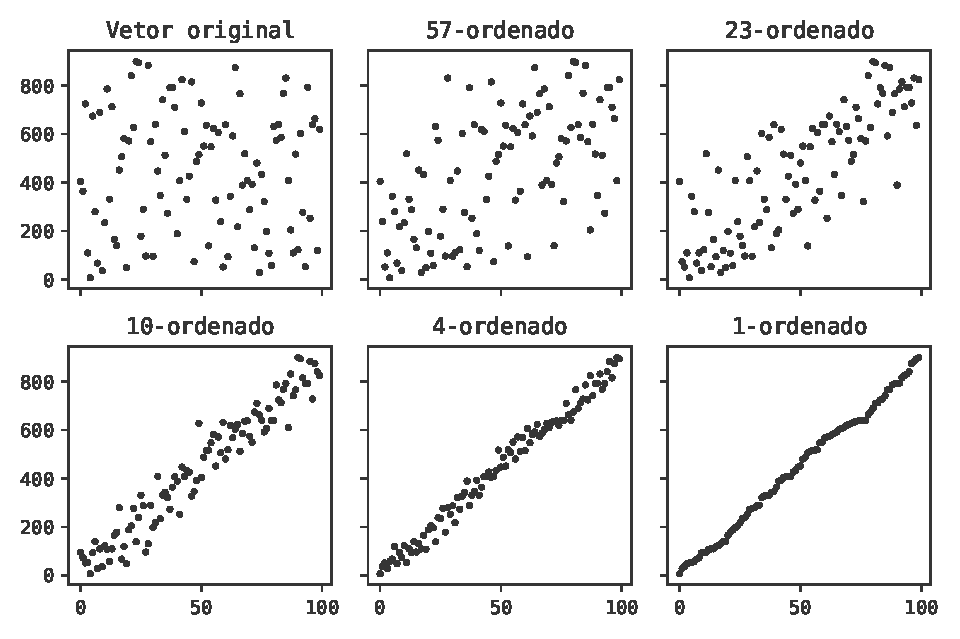
\includegraphics[scale=0.9]{figuras/pdf/shellsort.pdf}
\Fonte{Elaborado pelo autor}
\end{figure}

\section{Mergesort}
O Mergesort é um algoritmo de ordenação estável baseado na técnica de divisão e conquista, proposto por John von Neumann em 1945. Essa técnica consiste em um processo recursivo de três etapas:
\begin{enumerate}
    \item Divisão: divide-se o problema em instâncias menores do mesmo problema.
    \item Conquista: resolve-se cada uma das instâncias definidas na etapa anterior.
    \item Combinação: combinam-se as soluções para resolver o problema original.
\end{enumerate}

Enquanto as etapas de divisão e conquista consistem apenas em algumas operações aritméticas e duas chamadas recursivas, a de combinação requer um pouco mais de atenção. Nesse momento, tem-se dois vetores ordenados, e é necessário juntá-los em apenas um vetor também ordenado, em um processo chamado intercalação, que aqui será referido pelo termo em inglês \textit{merge}.

\subsection*{Intercalação de vetores ordenados}
A implementação da operação \textit{merge} é mostrada em linguagem C abaixo. Ela assume que $v[l..m - 1]$ e $v[m..r - 1]$ estão ordenados. O resultado é que $v[l..r - 1]$ também ficará em ordem. A função CopiaVetor, na linha 2, copia os $r - l$ elementos de $v[l..r - 1]$ para o vetor auxiliar $v\_aux[l..r - 1]$. Doravante, essa função será usada de forma similar, sem mais explicações.

\lstinputlisting[language=C]{codigos/aux/merge.txt}

\subsection*{O algoritmo Mergesort}
Este trabalho traz uma implementação dividida em dois métodos. O primeiro é apenas uma interface que segue o mesmo padrão de assinatura dos métodos de ordenação mostrados anteriormente, e é responsável por alocar e liberar a memória auxiliar, além de invocar o segundo método. O segundo é uma implementação recursiva do algoritmo que executa as três etapas da técnica já mencionada. A função AlocaVetor usa malloc para alocar um vetor com o tamanho especificado e verifica se a alocação ocorreu com sucesso.

\lstinputlisting[language=C]{codigos/sup/2_mergesort.txt}

\begin{figure}[H]
\Caption{\label{fig:mergesort}Ilustração do Mergesort aplicado ao vetor $[19,2,17,3,13,5,11,7]$.}
\centering
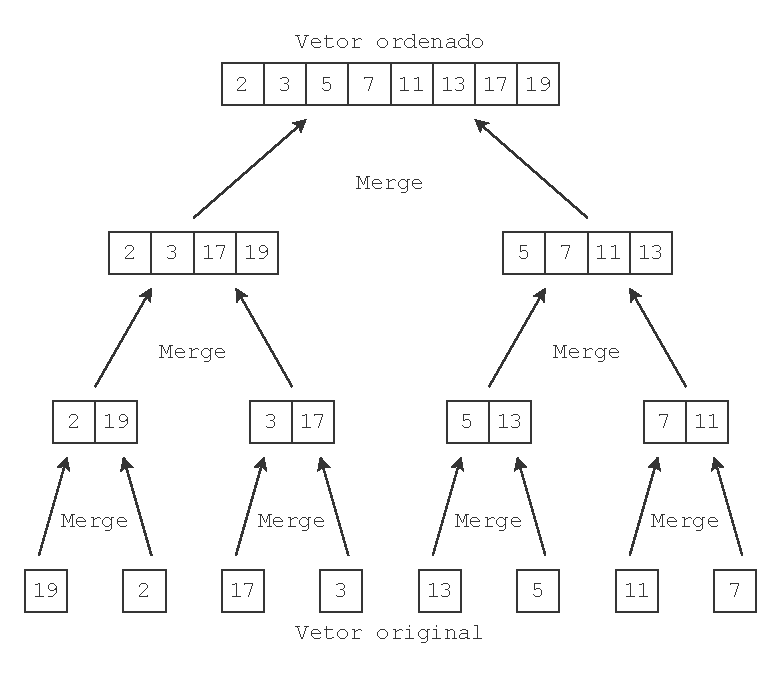
\includegraphics[scale=1.0]{figuras/pdf/mergesort.pdf}
\Fonte{Elaborado pelo autor}
\end{figure}

\subsection*{Corretude}
Observe que a base da recursão está bem definida, pois um vetor com menos de dois elementos já está ordenado. Note também que, em cada chamada, o vetor é dividido aproximadamente ao meio, e cada metade é ordenada recursivamente, sem deixar lacunas antes, entre ou depois de cada uma. Por fim, veja que a função Merge copia $v[l..r - 1]$ para $v\_aux[l..r - 1]$ e depois traz os elementos de volta para $v$, um por um, sempre escolhendo o menor que ainda não foi copiado. Como cada uma das etapas está correta, o Mergesort também está correto.

\subsection*{Desempenho}
Seja $T(n)$ o tempo necessário para ordenar um vetor de $n$ elementos utilizando o Mergesort. Temos então que:
\[
  T(n) = 
  \begin{cases}
      \Theta(1),              & n = 1    \\
      \underbrace{\Theta(1)}_{\text{Divisão}} + \underbrace{2T(n/2)}_{\text{Conquista}} + \underbrace{\Theta(n)}_{\text{Intercalação}}, & n > 1 
  \end{cases}
\]
Desta forma, podemos simplesmente dizer que para $n > 1$ e alguma constante $c$,
\[
  T(n) \;=\; 2T(n/2) + cn \;\;\;\Rightarrow\;\;\; T(n) \;=\; n\log_2 n + cn
\]
Portanto, o consumo de tempo do Mergesort é $\Theta(n\log_2 n)$. Já o de memória é $\Theta(n)$, devido ao vetor auxiliar utilizado.

\section{Heapsort}
O algoritmo Heapsort foi introduzido por J. W. J. Williams em 1964, no artigo \textit{Algorithm 232: Heapsort}, publicado na revista \textit{Communications of the ACM}. Como o próprio nome sugere, este algoritmo faz uso de uma estrutura de dados chamada \textit{heap}, mais especificamente um \textit{max-heap} binário.

\subsection*{\textit{max-heap} binário}
Um \textit{max-heap} binário -- de agora em diante referido apenas como \textit{heap} -- é uma árvore binária quase completa que satisfaz a propriedade de que o valor armazenado em um nó pai é maior ou igual ao valor de seus filhos. Uma árvore binária é considerada quase completa quando todos os seus níveis estão completamente preenchidos, exceto possivelmente o último, que deve ser preenchido da esquerda para a direita.

Convenientemente, essa árvore pode ser implementada em um vetor, de modo que cada posição do vetor represente um nó da árvore. Os filhos do nó na posição $i$ estão localizados nas posições $2i + 1$ e $2i + 2$, desde que essas posições sejam válidas.

\begin{figure}[H]
\Caption{\label{fig:maxheap}Exemplo de max-heap binário.}
\centering
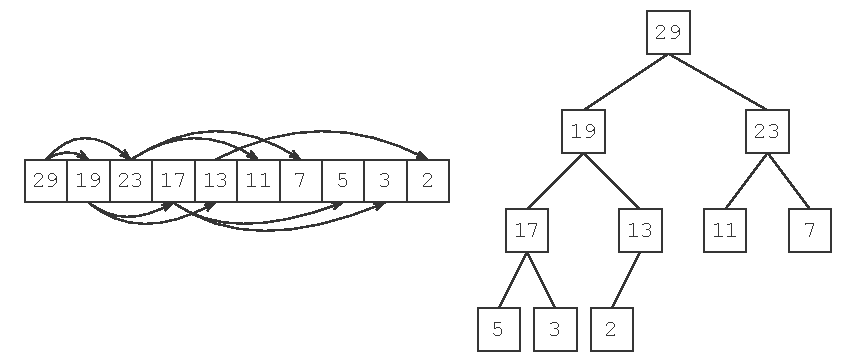
\includegraphics[scale=1.0]{figuras/pdf/max-heap.pdf}
\Fonte{Elaborado pelo autor.}
\end{figure}

\subsection*{Função Heapifica}
A função Heapifica será usada tanto para construir o \textit{heap} quanto para implementar o Heapsort em si. Ela é responsável por restaurar a propriedade de \textit{heap} em um ``quase \textit{heap}''. Um ``quase \textit{heap}'' é uma árvore em que apenas a raiz pode estar violando a propriedade de \textit{heap}. A ideia é simples: começando pela raiz, compara-se o nó atual com seu filho de maior valor; se o filho for maior, os dois são trocados de posição, e o processo é repetido com o novo nó até que a condição seja falsa ou uma folha seja atingida.
\lstinputlisting[language=C]{codigos/aux/heapifica.txt}

\subsection*{Construção do heap}
Considere o problema de transformar um vetor em um \textit{heap}. Para resolvê-lo, basta aplicar a operação Heapifica a todos os nós que não são folhas, da direita para a esquerda.
\lstinputlisting[language=C]{codigos/aux/constroi_heap.txt}

\subsection*{O algoritmo Heapsort}
O Heapsort começa transformando o vetor de entrada em um \textit{heap}. Após isso, o maior elemento estará na primeira posição. Sabendo disso, $v[0]$ é trocado com $v[n - 1]$. Neste momento, o maior elemento está na posição correta, e $v[0..n - 2]$ forma um “quase \textit{heap}”. Em seguida, a função Heapifica transforma $v[0..n - 2]$ em um \textit{heap}, e esse processo é repetido até que o \textit{heap} tenha apenas um elemento.
\lstinputlisting[language=C]{codigos/sup/3_heapsort.txt}

\subsection*{Desempenho}
A quantidade de operações que a função Heapifica executa quando invocada em um nó de altura $h$ é proporcional a $h$. Além disso, existem exatamente $2^M / 2^h$ nós com altura $h > 1$, onde $M = \lfloor \log_2 n \rfloor + 1$. Logo, a quantidade total de operações na construção do \textit{heap} é dada por:
\[
\sum_{h=2}^{M} h\left(\frac{2^M}{2^h}\right) \;=\; 2^M\cdot\sum_{h=2}^{M} h\left(\frac{1}{2}\right)^h \;\;<\;\; 2^M\cdot\sum_{h=1}^{\infty} h\left(\frac{1}{2}\right)^h \;=\; 2^{M+1} \;\;\approx\;\; 2n
\]
Portanto, o \textit{heap} é construído em tempo linear, \bigO{n}. Já a segunda parte do algoritmo, a partir da linha 3, executa aproximadamente
\[
\sum_{i=1}^{n-1} \log_2 i \;=\; \log_2 (n-1)! \;\;\leq\;\; n\log_2 n
\]
operações e, portanto, todo o algoritmo consome tempo proporcional a \bigO{n\log_2 n}.

\section{Quicksort}
O Quicksort é um algoritmo de ordenação que provavelmente é o mais amplamente utilizado. A versão básica foi desenvolvida em 1960 por C. A. R. Hoare e, desde então, tem sido estudado por muitas pessoas. O Quicksort é popular porque não é difícil de implementar, é um bom algoritmo de ordenação de uso geral e, em muitos casos, consome menos recursos do que qualquer outro método de ordenação \cite[p.115, tradução nossa]{book:58781}.

O algoritmo Quicksort é um método de ordenação não estável que funciona da seguinte maneira: particiona-se o vetor em dois segmentos, de modo que os menores elementos fiquem no primeiro e os maiores no segundo. Em seguida, o processo é repetido recursivamente em cada um dos segmentos, enquanto eles tiverem tamanho maior que um.

A escolha de um elemento pivô define quais elementos são considerados menores e quais são considerados maiores. As estratégias para escolha do pivô, bem como o processo de particionamento, são apresentados a seguir.

\subsection*{Particionamento}
Existem versões básicas do Quicksort que definem como pivô um elemento localizado em um índice fixo do intervalo, como, por exemplo, sempre escolher um dos extremos. Essa estratégia pode levar à complexidade \bigO{n^2} para entradas que já estejam ordenadas, além de empilhar cerca de $n$ chamadas recursivas, o que pode causar um estouro de pilha. Contudo, a versão do Quicksort apresentada neste trabalho já incorpora algumas otimizações. A função Particiona, apresentada a seguir, escolhe o pivô de forma pseudoaleatória.

\lstinputlisting[language=C]{codigos/aux/particiona.txt}

Na implementação da função Particiona mostrada acima, a função GeraNumeroAleatorioNoIntervalo utiliza a função \textit{rand}, presente na biblioteca padrão da linguagem C. O retorno da função Particiona é um índice $j$ tal que
\[
\begin{array}{ccc}
    l \leq j \leq r & \text{ e } & 
    \begin{cases}
        v[j] = piv\hat{o}\\
        v[k] \leq piv\hat{o}, & l \leq k < j \\
        v[k] > piv\hat{o}, & j < k \leq r
    \end{cases}
\end{array}
\]

\subsection*{O algoritmo Quicksort}
A implementação do algoritmo Quicksort apresentada a seguir é idêntica àquela encontrada em \cite[p.90]{book97338b4c}. Ela traz duas melhorias em relação à implementação básica. A primeira consiste em sempre tratar primeiro o menor dos segmentos gerados pela função Particiona, garantindo que a altura da pilha de recursão seja, no máximo, $\log_2 n$. A segunda é a eliminação de uma das chamadas recursivas, que é transformada em uma iteração, convertendo o algoritmo em uma recursão de cauda.

\lstinputlisting[language=C]{codigos/sup/4_quicksort.txt}

\subsection*{Desempenho}
O pior caso do Quicksort tem complexidade \bigO{n^2} e ocorre quando a função Particiona retorna sempre, ou quase sempre, um índice $j$ muito próximo de $l$ ou $r$. Isso acontece, por exemplo, quando todos os elementos do vetor são iguais. Já o melhor caso tem complexidade \bigO{n\log_2 n} e ocorre quando $j$ está próximo do ponto médio entre $l$ e $r$ em todas as chamadas recursivas.

Em média, a complexidade desta versão aleatorizada do Quicksort é proporcional a \bigO{n\log_2 n}. Esse resultado pode ser demonstrado por meio do cálculo do valor esperado do número de comparações realizadas na linha 5 da função Particiona, conforme apresentado em \cite[p.180–184]{Cormen2009}. Para isso, observe que a probabilidade de os elementos $v[i]$ e $v[j]$ serem comparados durante a execução do algoritmo é dada por:
\[
P_{ij} = \dfrac{2}{j - i + 1}
\]
Seja $X$ a variável aleatória que representa a quantidade total de comparações feitas. Assim, sendo $k = j - i$, o valor esperado de $X$ é:
\[
\begin{array}{c c l}
    E[X] & = & \displaystyle\nsum_{i = 0}^{n - 2}\nsum_{j = i + 1}^{n - 1} \dfrac{2}{j - i + 1}\\[16pt]
         & = & \displaystyle\nsum_{i = 0}^{n - 2}\nsum_{k = 1}^{n - i - 1} \dfrac{2}{k + 1}\\[16pt]
         & < & \displaystyle\nsum_{i = 0}^{n - 2}\nsum_{k = 1}^{n} \dfrac{2}{k}\\
         & < & 2(n - 1)\ln n\\
         & = & \left(\dfrac{2(n - 1)}{\log_2 \mathrm{e}}\right)\log_2 n
\end{array}
\]

\section{Métodos híbridos}
Esta seção apresenta dois algoritmos de ordenação híbridos, assim chamados por combinarem dois ou mais dos algoritmos discutidos anteriormente.

\subsection{Quicksort com Inserção}
Este algoritmo combina a eficiência do Quicksort para vetores grandes com a do Insercao para vetores pequenos e quase ordenados, como ilustra a Figura \ref{fig:quicksort-insercao}. Ele consiste em duas etapas: a primeira é um Quicksort que ignora subvetores com tamanho menor ou igual a $16$; a segunda é a aplicação do Insercao a todo o vetor. Observe que, ao final da primeira etapa, cada elemento estará, no máximo, a $16$ posições de sua posição correta, de modo que o Insercao executará em tempo linear para finalizar a ordenação.

\begin{figure}[H]
\Caption{\label{fig:quicksort-insercao}Número médio de movimentações realizadas pelos algoritmos Quicksort e Insercao em vetores gerados de forma pseudoaleatória.}
\centering
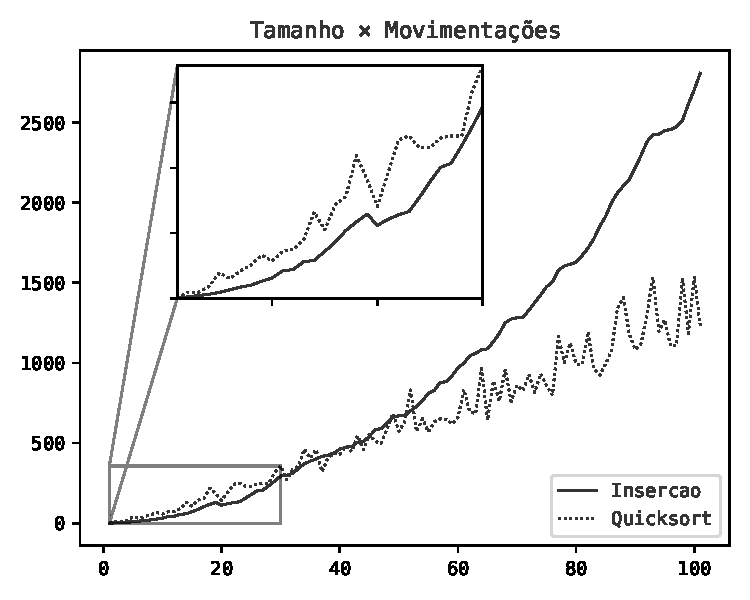
\includegraphics{figuras/pdf/quicksort-insercao.pdf}
\Fonte{Elaborado pelo autor}
\end{figure}

\lstinputlisting[language=C]{codigos/sup/5_quicksort_i.txt}

\subsection{Introsort}
O algoritmo Introsort foi introduzido em \cite{musser1997introspective} e é atualmente utilizado na implementação do método \textit{sort} da biblioteca padrão da linguagem C++.

\subsection*{Outro método de particionamento}
O Introsort controla a altura da pilha de recursão de maneira diferente daquela utilizada no Quicksort, o que possibilita o uso de outro método de particionamento que, como mostra a Figura \ref{fig:particiona_1_2}, realiza menos trocas. Além disso, o elemento pivô é escolhido de forma distinta. A função MoveMedianaFim posiciona, na última posição do vetor, a mediana entre os elementos $v[l]$, $v[(l + r)/2]$ e $v[r]$. Essa estratégia de escolha do pivô é conhecida como ``mediana de três''.
\lstinputlisting[language=C]{codigos/aux/particiona2.txt}

\begin{figure}[H]
\Caption{\label{fig:particiona_1_2}Número médio de trocas realizadas pelos métodos Particiona e Particiona2 em vetores gerados de forma pseudoaleatória.}
\centering
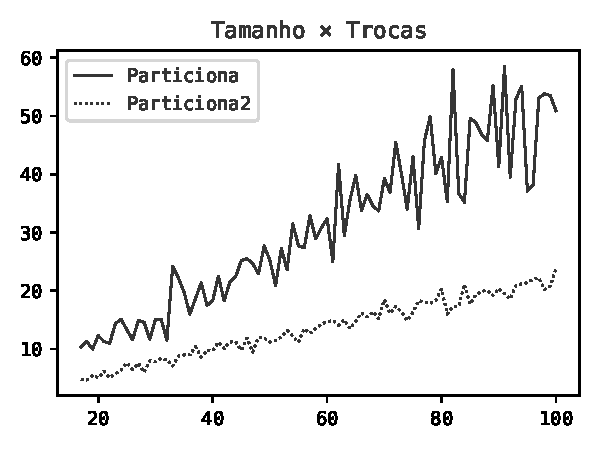
\includegraphics{figuras/pdf/particiona_1_2.pdf}
\Fonte{Elaborado pelo autor}
\end{figure}

\subsection*{O algoritmo Introsort}
A ideia consiste em evitar o pior caso do Quicksort utilizando o Heapsort quando o tamanho da pilha de recursão atinge o valor $\lfloor2\log_2 n\rfloor$. Dessa forma, como o Heapsort possui complexidade no pior caso linearítmica, o pior caso do Introsort é \bigO{n\log_2 n}. Além disso, assim como no algoritmo anterior, o Insercao é utilizado para concluir a ordenação.
\lstinputlisting[language=C]{codigos/sup/6_introsort.txt}

\chapter{Ordenação em tempo linear}\label{cap:lineares}
Este capítulo apresenta três métodos de ordenação que não se baseiam diretamente em comparações e que, sob determinados critérios, realizam a ordenação em tempo linear.

\section{Countingsort}
O algoritmo Countingsort baseia-se na contagem do número de ocorrências de cada elemento na entrada para determinar suas posições na saída. Foi introduzido por Harold H. Seward em 1954 e é particularmente eficiente quando os valores dos elementos a serem ordenados pertencem a um intervalo pequeno e conhecido. A implementação apresentada a seguir assume que o vetor de entrada não contém elementos negativos e que o maior elemento é suficientemente pequeno para permitir a criação de um vetor com esse tamanho.
\lstinputlisting[language=C]{codigos/lin/1_countingsort.txt}

\section{Bucketsort}
O Bucketsort é um algoritmo de ordenação descrito por John W. Tukey em 1944. Ele se baseia na distribuição dos elementos em diferentes grupos, chamados ``buckets'', cujos conteúdos são ordenados individualmente. Por fim, os buckets são concatenados, resultando em um vetor ordenado.

\begin{figure}[H]
\Caption{\label{fig:buckets}Ilustração do intervalo correspondente a cada bucket, em que $B_i$ representa o $i$-ésimo bucket e $M$ é o maior elemento que pode existir no vetor.}
\centering
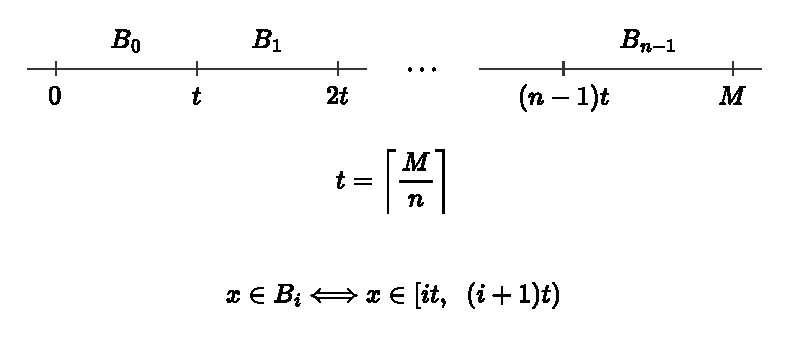
\includegraphics[scale=1.0]{figuras/pdf/buckets.pdf}
\Fonte{Elaborado pelo autor.}
\end{figure}

Caso os elementos do vetor de entrada estejam distribuídos de forma uniforme no intervalo $[0, M]$, é esperado que cada bucket contenha uma quantidade constante de elementos, de modo que o algoritmo Bucketsort execute em tempo linear. No entanto, não se sabe previamente quantos elementos cada bucket armazenará durante a execução. Por isso, cada bucket foi implementado como uma estrutura de crescimento dinâmico, utilizando listas ligadas. Além disso, o método InsereOrdenado foi desenvolvido de forma semelhante ao algoritmo Insercao.

\lstinputlisting[language=C]{codigos/lin/2_bucketsort.txt}

\section{Radixsort}
O algoritmo Radixsort é um método de ordenação estável para números naturais, que funciona da seguinte maneira: dado um vetor de $n$ números naturais com $d$ dígitos cada, utiliza-se um algoritmo de ordenação estável para ordená-los pelo dígito menos significativo, depois pelo segundo menos significativo e assim por diante. O Radixsort depende da estabilidade do algoritmo auxiliar para garantir a correção do processo. Se existirem $k$ valores possíveis para cada dígito, e o algoritmo auxiliar ordenar em tempo proporcional a \bigO{n + k}, então o Radixsort terá complexidade \bigO{d(n + k)}, ou seja, complexidade linear.

A seguir, são apresentadas as duas versões do Radixsort que foram implementadas: uma utilizando uma adaptação do algoritmo Countingsort e outra, uma adaptação do Bucketsort. Como o objetivo deste trabalho é simplesmente ordenar números naturais em base decimal, a função Digito(x, p), utilizada em ambas as versões, assume que $p = 10^r$ e retorna $\lfloor x / p \rfloor \mod 10$, ou seja, o dígito de $x$ que está na posição $r + 1$, da direita para a esquerda.

\subsection*{Radixsort com Countingsort}
A principal diferença em relação ao algoritmo Countingsort apresentado anteriormente é que o vetor de \textit{cont} possui apenas $10$ posições e armazena as ocorrências dos dígitos de $0$ a $9$, extraídos das posições indicadas por $p$ nos elementos do vetor $v$.
\lstinputlisting[language=C]{codigos/lin/3_radixsort_c.txt}

\subsection*{Radixsort com Bucketsort}
Em comparação com o algoritmo Bucketsort, a lista de buckets contém apenas $10$ posições, uma para cada valor possível de dígito. Por exemplo, se o dígito indicado por $p$ em $v[i]$ for igual a $5$, então $v[i]$ é colocado no bucket $5$. Observe que é suficiente inserir cada elemento diretamente no início de cada bucket, ou seja, como primeiro elemento da lista ligada, sem a necessidade de manter a lista ordenada.
\lstinputlisting[language=C]{codigos/lin/4_radixsort_b.txt}

\chapter{Análise empírica}\label{cap:analise-empirica}
Este capítulo tem como objetivo analisar empiricamente todos os algoritmos de ordenação apesentados anteriormente, comparando a análise teórica com os resultados obtidos na prática, no que diz respeito ao tempo de execução, número de comparações e número de movimentações.

\section{Preliminares}
Nesta seção, descreve-se o ambiente de desenvolvimento, indicando o hardware e os softwares utilizados na implementação dos algoritmos e na execução dos testes. Também é apresentada a organização do projeto em diretórios e arquivos. Além disso, são feitas definições necessárias para o melhor entendimento das seções seguintes. Por fim, descreve-se o que foi coletado e como essa coleta foi realizada.

\subsection{Ambiente de desenvolvimento}
Para a implementação dos algoritmos e execução dos testes foi utilizado o notebook descrito na Tabela \ref{tab:hardware-and-softwares}. Todos os algoritmos e funções auxiliares foram implementados com a linguagem de programação C. As linguagens de programação Bash e Python foram utilizadas de forma secundária para automatização dos testes e geração de gráficos, respectivamente. O hardware, softwares e versões utilizados são especificados na tabela \ref{tab:hardware-and-softwares}.

\begin{table}[H]
    \centering
    \Caption{\label{tab:hardware-and-softwares}Hardware e softwares utilizados}
    \begin{tabular}{ | c | l | l | }
        \hline
        Tipo                      & Componente                & Produto                          \\
        \hline
        \multirow{3}{*}{Hardware} & Modelo                    & Avell A65i                       \\
                                  & Processador               & 13th Gen Intel® Core™ i9-13900HX \\
                                  & Cache                     & 36 MB Intel® Smart Cache         \\
                                  & Memória principal         & 64.0 GiB                         \\
        \hline
        \multirow{4}{*}{Software} & Sistema operacional       & Linux Ubuntu 24.04.3 LTS         \\
                                  & Editor de texto           & Microsoft Visual Studio Code     \\
                                  & Compilador C              & GNU Compiler Collection GCC      \\
                                  & Linguagens de programação & C, Bash e Python                 \\
        \hline
    \end{tabular}
\end{table}

\subsection{Organização do código fonte}
A figura \ref{fig:projeto-ordenacao} ilustra a forma como código fonte do projeto foi organizado, enquanto que a tabela \ref{tab:projeto-ordenacao} dá uma breve descrição de cada arquivo.

\begin{figure}[H]
\Caption{\label{fig:projeto-ordenacao}Árvore de diretórios e arquivos do projeto}
\centering
\begin{forest}
    for tree={font=\ttfamily, grow'=0,
    folder indent=.9em, folder icons,
    edge=densely dotted}
    [
        [graficos
            [graficos.ipynb, is file]
        ]
        [scripts
            [testes.sh, is file]
        ]
        [src
            [main.c, is file]
            [ordenacao.c, is file]
            [ordenacao.h, is file]
        ]
        [.gitignore, is file]
        [README.md, is file]
    ]
\end{forest}
\vspace{3pt}
\Fonte{Elaborado pelo autor. Acesso público em https://github.com/jbrenorv/ordenacao}
\end{figure}

\begin{table}[H]
    \centering
    \Caption{\label{tab:projeto-ordenacao}Descrição dos arquivos do projeto}
    \begin{tabular}{ | c | l | }
        \hline
        Arquivo        & Descrição                                                       \\
        \hline
        graficos.ipynb & Arquivo exportado do notebook criado no Google Colab            \\
        testes.sh      & Implementa script em Bash para execução automatizada dos testes \\
        main.c         & Implementa a função principal                                   \\
        ordenacao.c    & Implementa os algoritmos de ordenação e funções utilitárias     \\
        ordenacao.h    & Declara os protótipos dos algoritmos e funções utilitárias      \\
        .gitignore     & Declara diretórios e arquivos que o Git deve ignorar            \\
        README.md      & Documenta o projeto com instruções de execução dos testes       \\
        \hline
    \end{tabular}
\end{table}

\subsection{Tipos de vetores}
Além do tamanho do vetor, a forma como os elementos estão dispostos inicialmente pode interferir no tempo e na quantidade de operações que cada algoritmo executa. Pensando nisso, com o objetivo de analisar como cada algoritmo se comporta para diferentes tipos de entrada, foram considerados três tipos de vetores nos testes, como mostra a tabela \ref{tab:tipos-de-vetores}.

\begin{table}[H]
    \centering
    \Caption{\label{tab:tipos-de-vetores}Tipos de vetores}
    \begin{tabular}{ | c | l | }
        \hline
        Tipo   & Descrição                                \\
        \hline
        1      & Vetores já ordenados em ordem crescente  \\
        2      & Vetores ordenados em ordem decrescente   \\
        3      & Vetores gerados de forma pseudoaleatória \\
        \hline
    \end{tabular}
\end{table}

\subsection{Dados coletados}
Esta seção visa apenas apresentar e definir quais dados foram coletados. A próxima seção descreve com mais detalhes como a coleta foi realizada. Para cada combinação de algoritmo, tamanho e tipo de vetor, foi registrado o número de comparações, o número de movimentações e o tempo de execução. Essas três métricas são definidas na tabela \ref{tab:dados-coletados}.

Obter essas informações de cada algoritmo é importante para sabermos na prática como eles se comportam para diferentes configurações de entrada. Por exemplo, um algoritmo que executa muitas movimentações pode não ser adequado em um cenário em que mudar os registros de posição seja uma operação muito lenta.

\begin{table}[H]
    \centering
    \Caption{\label{tab:dados-coletados}Dados coletados e suas definições}
    \begin{tabular}{ | c | l | }
        \hline
        Dado                    & Definição                                                     \\
        \hline
        Número de comparações   & \makecell[l]{Uma comparação ocorre quando um elemento do      \\
                                               vetor é comparado com outro elemento do vetor ou \\
                                               com outra variável do programa}                  \\
        Número de movimentações & \makecell[l]{Uma movimentação ocorre sempre que um valor é    \\
                                               atribuído a um elemento do vetor ou um elemento  \\
                                               do vetor é atribuído a uma outra variável}       \\
        Tempo de execução       & \makecell[l]{Tempo decorrido entre o início e o fim da        \\
                                               execução do algoritmo em segundos}               \\
        \hline
    \end{tabular}
\end{table}

\subsection{Metodologia de coleta}
\subsubsection{Entrada}
A função principal é o ponto de entrada para qualquer programa escrito em linguagem de C. De uma forma mais técnica, ao compilar e linkar o código fonte do projeto, obtém-se um arquivo binário executável que, ao ser executado, invoca a função principal para iniciar a execução do processo. Essa função recebe dois argumentos quando invocada. O primeiro é um número inteiro comumente chamado de argc, que indica a quantidade de parâmetros recebidos. Já o segundo é uma lista de vetores de caracteres comumente chamado de argv, que são os parâmetros em si. O primeiro parâmetro é sempre o nome do arquivo executável ou o caminho absoluto até ele. A tabela \ref{tab:main-parametros} indica os parâmetros adicionais esperados.
\begin{table}[H]
    \centering
    \Caption{\label{tab:main-parametros}Parâmetros da função principal}
    \begin{tabular}{ | c | l | }
        \hline
        Posição (argv) & Parâmetro esperado                                      \\
        \hline
        0              & Nome ou caminho para o arquivo executável               \\
        1              & Nome do arquivo onde deve ser escrito os resultados     \\
        2              & Número representando o tamanho do vetor                 \\
        3              & Número igual a 1, 2 ou 3, representando o tipo do vetor \\
        4              & Número representando número da execução                 \\
        \hline
    \end{tabular}
\end{table}

O último parâmetro, que indica o número da execução, é explicado na subseção \ref{subsection:Testes}, que apresenta como os testes foram executados.

\subsubsection{Processamento}
O processamento consiste na execução sequencial das etapas necessárias para realizar os experimentos definidos neste trabalho. O pseudocódigo apresentado a seguir oferece uma visão de alto nível do fluxo executado pela função principal, desde a leitura dos parâmetros de entrada até o registro dos resultados obtidos. Optou-se por essa forma de apresentação para destacar a lógica geral do procedimento e evitar a exibição detalhada de trechos de código que não contribuem significativamente para a compreensão do funcionamento do sistema.

\begin{algorithm}[H]
    \caption{Função principal}\label{alg-main:cap}
    \DontPrintSemicolon
    \Entrada{A tupla $(S, N, T, E)$ representado os parâmetros listados na tabela \ref{tab:main-parametros}}
    \Inicio{
        $F \gets$ Abre arquivo $S$\;
        $O \gets$ Aloca vetor de tamanho $N$ com valores de acordo com o tipo $T$\;
        $V \gets$ Aloca vetor de tamanho $N$\;
        $L \gets$ Cria lista de pares de algoritmos\footnote{O primeiro elemento é o algoritmo original e o segundo é a versão modificada para obter o número de comparações e movimentações.}\;
        \Para{cada par $(A, A') \in L$}{
            $V \gets$ Cópia de $O$\;
            $t \gets$ Executa $A$ em $V$\footnote{Obtendo o tempo de execução $t$ em segundos.}\;
            $V \gets$ Cópia de $O$\footnote{Neste ponto $V$ está ordenado, então é necessário resetar para o vetor original.}\;
            $(c, m) \gets$ Executa $A'$ em $V$\footnote{Obtendo o número de comparações $c$ e movimentações $m$.}\;
            Adiciona em $F$ uma linha com os resultados\footnote{Precisamente, a linha contêm o nome do algoritmo, o tamanho do vetor, o tipo do vetor, o número da execução, o número de comparações, o número de movimentações e o tempo de execução.}\;
        }
        Libera a memória alocada e fecha o arquivo $F$\;
    }
\end{algorithm}

\subsubsection{Exemplo de saída}
Se após compilar e linkar o código C, o arquivo executável resultante se chamar a.out, o comando a ser executado a partir de um Terminal Linux, aberto no mesmo diretório do executável, poderia ser, por exemplo:
\lstinputlisting[language=bash]{codigos/aux/_bash.txt}
Neste caso, seria gerado um vetor de forma pseudoaleatória (tipo 3) de tamanho 1000 e os resultados seriam escritos no arquivo saida.csv. Com exceção do cabeçalho, o conteúdo do arquivo saida.csv é representado na tabela \ref{tab:exemplo-saida}. Além disso, a coluna do tempo pode conter valores diferentes.
\begin{table}[H]
    \centering
    \Caption{\label{tab:exemplo-saida}Exemplo de saída}
    \begin{tabular}{ | c | l | l | l | l | l | l | }
        \hline
        Algo.        & Tam. & Tipo & Exec. & Comp.  & Movi.  & Tempo (s) \\
        \hline
        Bolha        & 1000 & 2    & 1     & 499497 & 770538 & 0.004037  \\
        Coquetel     & 1000 & 2    & 1     & 388815 & 770538 & 0.003501  \\
        Selecao      & 1000 & 2    & 1     & 499500 & 2958   & 0.000543  \\
        Insercao     & 1000 & 2    & 1     & 257838 & 258844 & 0.000163  \\
        Shellsort    & 1000 & 2    & 1     & 13061  & 20296  & 0.000111  \\
        Mergesort    & 1000 & 2    & 1     & 8717   & 19302  & 0.000098  \\
        Heapsort     & 1000 & 2    & 1     & 8772   & 14040  & 0.000104  \\
        Quicksort    & 1000 & 2    & 1     & 10345  & 20325  & 0.000103  \\
        QuicksortI   & 1000 & 2    & 1     & 12107  & 17646  & 0.000072  \\
        Introsort    & 1000 & 2    & 1     & 14047  & 9620   & 0.000078  \\
        Countingsort & 1000 & 2    & 1     & 0      & 2000   & 0.155960  \\
        Bucketsort   & 1000 & 2    & 1     & 1050   & 4050   & 0.000037  \\
        RadixsortC   & 1000 & 2    & 1     & 0      & 18000  & 0.000022  \\
        RadixsortB   & 1000 & 2    & 1     & 0      & 45000  & 0.000034  \\
        \hline
    \end{tabular}
\end{table}

\subsubsection{Testes}\label{subsection:Testes}
Neste ponto o código implementado em linguagem C está pronto para ser invocado com diferentes parâmetros de entrada. Para automatizar este processo, foi criado um script em linguagem Bash. Este script segue os seguintes passos:
\begin{enumerate}
    \item Compilação do código C e inicialização do arquivo CSV de saída.
    \item Geração dos tamanhos.
    \item Três execuções para cada tamanho e tipo de vetor.
\end{enumerate}

Optou-se por realizar três execuções por tamanho e tipo de vetor para reduzir o impacto de variações ocasionais no tempo de execução, como pequenas flutuações no uso da CPU. Esse número foi escolhido por ser suficiente para obter uma média representativa sem tornar a coleta de dados muito demorada.

Os tamanhos gerados são melhores descritos na tabela \ref{tab:tamanhos}. Foram considerados ao todo $37$ tamanhos entre $10^4$ e $10^8$, inclusive. Além disso, cada tamanho foi usado três vezes para cada um dos três tipos, totalizando $333$ chamadas aos algoritmos.
\begin{table}[H]
    \centering
    \Caption{\label{tab:tamanhos}Geração de tamanhos}
    \begin{tabular}{ | c | l | l | l | c | }
        \hline
        \multicolumn{2}{ | c | }{Intervalo} & \multirow{2}{*}{Incremento} & \multirow{2}{*}{Subtotal} & \multirow{2}{*}{Total} \\
        \cline{1-2}
        Início     & Fim        &        &    &                     \\
        \hline
        $10^4$     & $10^5 - 1$ & $10^4$ & 9  & \multirow{4}{*}{37} \\
        $10^5$     & $10^6 - 1$ & $10^5$ & 9  &                     \\
        $10^6$     & $10^7 - 1$ & $10^6$ & 9  &                     \\
        $10^7$     & $10^8$     & $10^7$ & 10 &                     \\
        \hline
    \end{tabular}
\end{table}

\section{Métodos inferiores}
Os quatro algoritmos classificados neste trabalho como inferiores possuem, como já detalhado em capítulos anteriores, complexidade temporal quadrática no tamanho do vetor de entrada. Eles recebem essa denominação por apresentarem, de acordo com a análise de complexidade apresentada no Capítulo \ref{cap:inferiores}, essa ordem de crescimento. Entretanto, embora todos apresentem a mesma complexidade assintótica, os testes práticos demonstraram que eles possuem desempenhos distintos.

Como o tempo de execução desses algoritmos apresenta crescimento quadrático à medida que o tamanho da entrada aumenta, o tamanho máximo do vetor utilizado foi $n=10^5$. Este tamanho foi considerado razoável para a observação dos resultados esperados, mantendo um tempo de execução viável para os testes.

\subsection{Tempo de execução}
O gráfico a seguir apresenta os resultados de tempo de execução obtidos ao se executar algoritmos de ordenação inferiores.

\begin{figure}[H]
\Caption{\label{fig:inferiores-tempo}Métodos inferiores – Tamanho × Tempo (em segundos).}
\centering
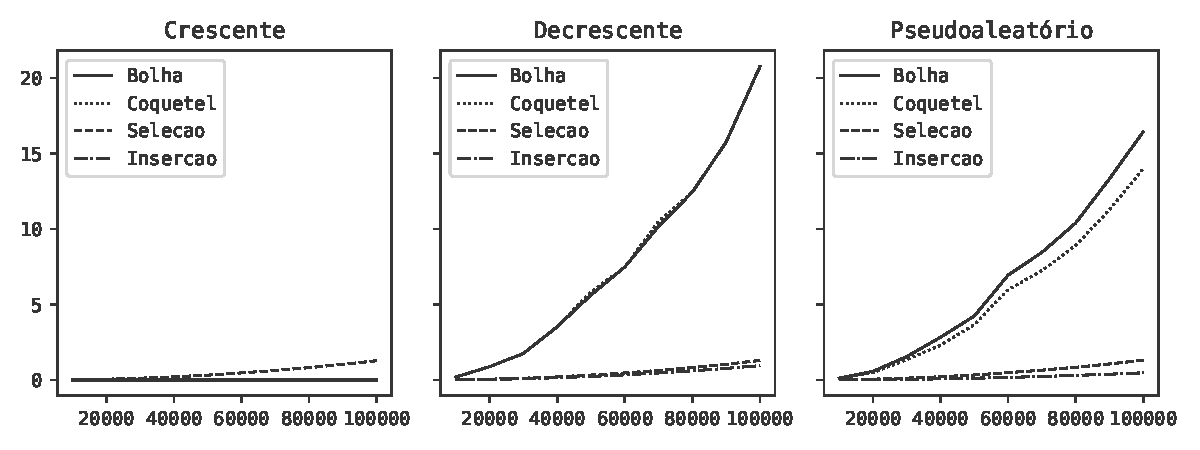
\includegraphics[scale=0.787]{figuras/pdf/inferiores.tempo.pdf}
\Fonte{Elaborado pelo autor}
\end{figure}

Para vetores já ordenados em ordem crescente, como esperado, apenas o algoritmo Selecao chegou a consumir mais de $1s$. Todos os demais algoritmos executaram apenas uma iteração e concluíram suas execuções, o que resultou em um tempo de consumo praticamente nulo.

O pior caso de todos os algoritmos fica evidente para vetores que, inicialmente, estão em ordem decrescente. Curiosamente, no entanto, os algoritmos Bolha e Coquetel se mostraram significativamente mais lentos que o Insercao e o Selecao. O motivo para esse desempenho será detalhado nas próximas seções, onde comparamos o número de comparações e movimentações que cada algoritmo realizou para este tipo de vetor.

Por fim, buscando observar o comportamento geral dos algoritmos, analisamos os vetores gerados de forma pseudoaleatória. Os algoritmos Bolha e Coquetel apresentaram uma leve melhora de desempenho, sendo o Coquetel ligeiramente mais rápido. Isso ocorre porque a iteração de retorno do Coquetel permite que elementos menores atinjam suas posições finais mais rapidamente do que no Bolha. Já os algoritmos Selecao e Insercao foram significativamente mais rápidos, com o Insercao apresentando o melhor resultado geral. Vale notar que o Selecao manteve praticamente o mesmo tempo de execução, independentemente do tipo de vetor. Tal fato se deve à sua característica de sempre executar uma quantidade fixa e quadrática de comparações, enquanto realiza um número mínimo de trocas. Dessa forma, o número de movimentações do Selecao é desprezível no tempo final de execução, o que o torna uma boa escolha para casos em que o vetor possui poucos elementos e a operação de movimentação tem um custo computacional elevado.


\subsection{Comparações}
O gráfico da Figura \ref{fig:inferiores-comparacoes} a seguir, exibe a relação entre o número de comparações e o tamanho do vetor para cada tipo de vetor analisado.

\begin{figure}[H]
\Caption{\label{fig:inferiores-comparacoes}Métodos inferiores – Tamanho × Comparações.}
\centering
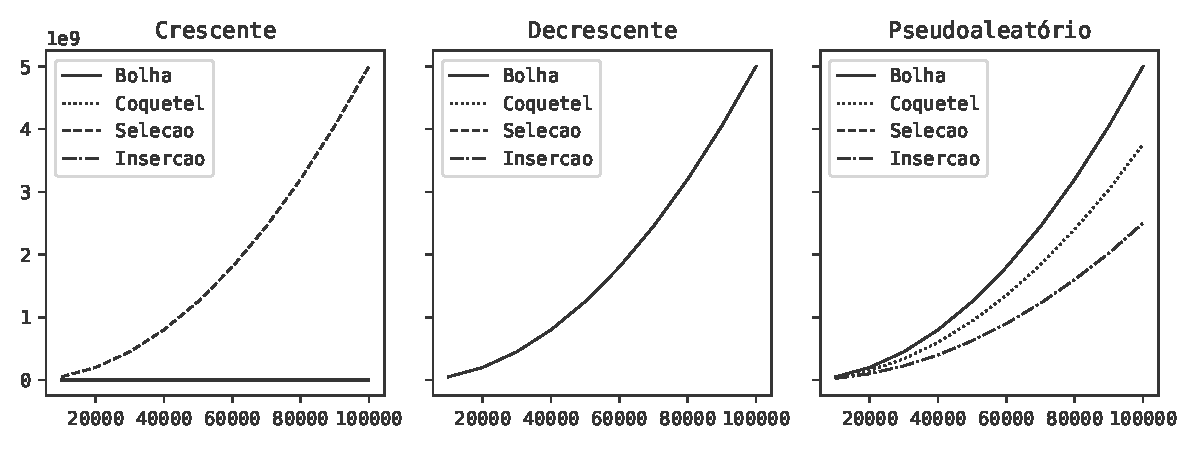
\includegraphics[scale=0.787]{figuras/pdf/inferiores.comparacoes.pdf}
\Fonte{Elaborado pelo autor}
\end{figure}

Para vetores em ordem crescente, como esperado, apenas o algoritmo Selecao executou uma quantidade quadrática de comparações. Os demais algoritmos, por outro lado, executaram uma quantidade linear de comparações, pois levaram apenas uma iteração externa para identificar que o vetor já se encontrava ordenado.

A análise teórica indicava que os algoritmos de ordenação inferiores apresentavam seu pior caso em comum: o vetor ordenado em ordem decrescente. Além disso, ela mostrava que esses algoritmos executam exatamente a mesma quantidade de comparações para esse tipo de vetor. Os testes práticos confirmaram essa conclusão, como é claramente demonstrado no gráfico.

No caso geral, com os vetores gerados de forma pseudoaleatória, pode-se observar que os algoritmos Bolha e Selecao permaneceram praticamente empatados em termos de número de comparações. O algoritmo Insercao demonstrou o melhor resultado, sendo aquele que necessitou do menor número de comparações para finalizar sua execução e garantir um vetor ordenado. Já o Coquetel ficou em um meio-termo, mostrando-se razoavelmente superior ao Bolha e ao Selecao nesse quesito. Sua vantagem reside no fato de que cada iteração externa coloca dois elementos em suas posições finais, além de aproximar os demais elementos de suas posições corretas em pelo menos uma posição.

\subsection{Movimentações}
O gráfico da Figura \ref{fig:inferiores-movimentacoes} a seguir, exibe a relação entre o número de movimentações e o tamanho do vetor para cada tipo de vetor analisado.

\begin{figure}[H]
\Caption{\label{fig:inferiores-movimentacoes}Métodos inferiores – Tamanho × Movimentações.}
\centering
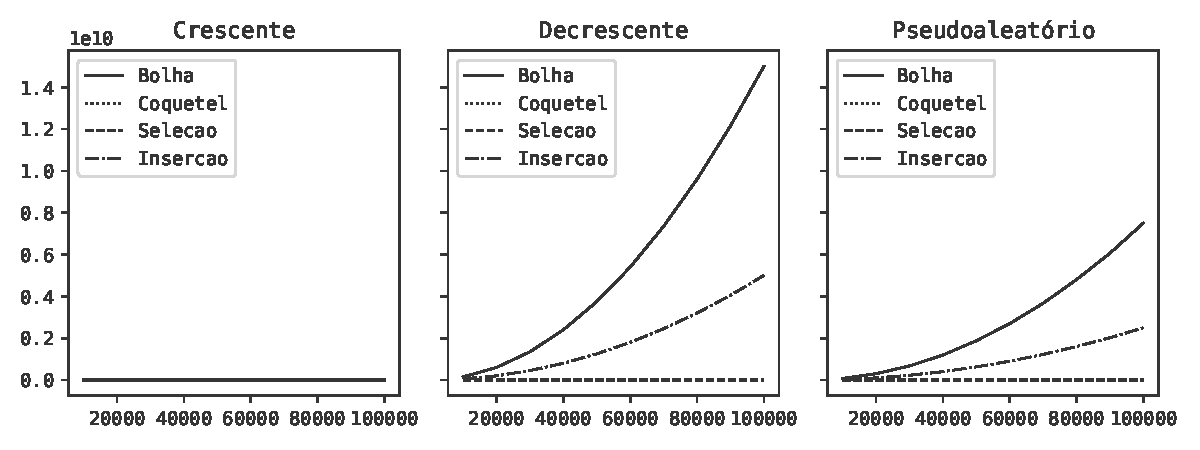
\includegraphics[scale=0.787]{figuras/pdf/inferiores.movimentacoes.pdf}
\Fonte{Elaborado pelo autor}
\end{figure}

Observe que, na prática, independentemente do tipo do vetor, os algoritmos Bolha e Coquetel possuem o mesmo desempenho com relação ao número de movimentações.

Neste ponto, pode-se estabelecer uma boa explicação para o Insercao ter apresentado o menor tempo de execução. Dentre todos os algoritmos inferiores, ele é o que melhor consegue equilibrar o número de comparações e movimentações. Ou seja, ele não possui extremos; enquanto o Bolha e o Coquetel geralmente executam muitas comparações e movimentações, e o Selecao executa muitas comparações e poucas movimentações, o Insercao permanece em um meio-termo. Essa característica o favorece, resultando em um tempo de execução menor que os demais para todos os tipos de vetores.

Quando o assunto é número de movimentações, o Selecao é o algoritmo mais eficiente. Isso ocorre porque ele executa sempre o número mínimo de trocas, garantindo que cada troca posicione pelo menos um elemento em sua posição definitiva. Dessa forma, ele realiza \bigO{n} movimentações, como fica evidente nos gráficos da Figura \ref{fig:selecao-movimentacoes} para todos os tipos de vetores. É importante notar que cada troca executa $3$ movimentações. Observe também que, para vetores decrescentes, cada troca posiciona dois elementos em suas posições finais.

\begin{figure}[H]
\Caption{\label{fig:selecao-movimentacoes}Selecao – Tamanho × Movimentações.}
\centering
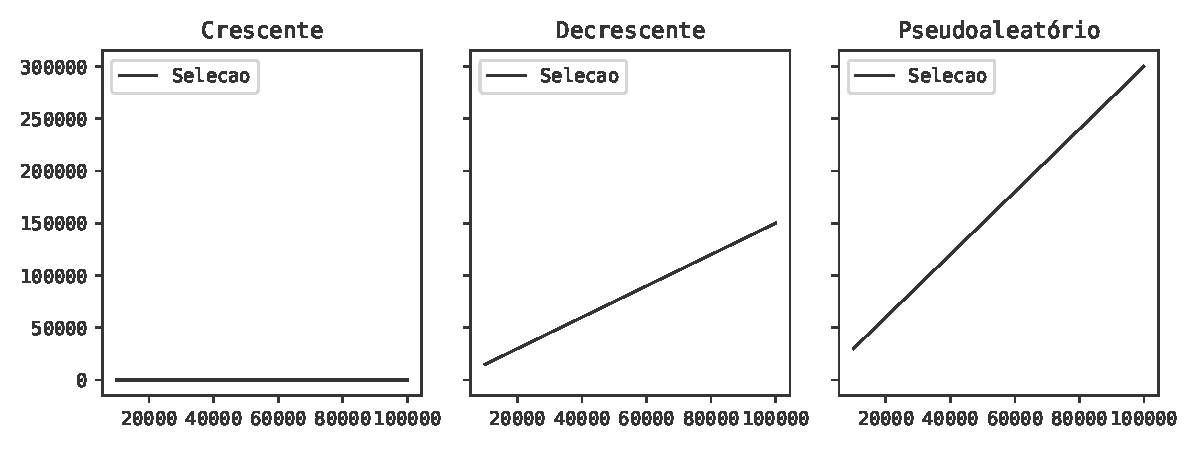
\includegraphics[scale=0.787]{figuras/pdf/selecao.movimentacoes.pdf}
\Fonte{Elaborado pelo autor}
\end{figure}

\section{Métodos superiores}
Os quatro algoritmos classificados como superiores são aqueles que possuem complexidade de tempo de ordem \bigO{n \log n}. Tal complexidade permite a realização de testes com vetores de tamanho consideravelmente maiores do que os utilizados para os algoritmos inferiores, razão pela qual foram testados com vetores cujo tamanho varia de $10^4$ a $10^8$.

\subsection{Tempo de execução}
Foram gerados dois gráficos para apresentar os resultados de tempo de execução. O primeiro, na Figura \ref{fig:superiores1e7-tempo}, mostra os resultados com o tamanho dos vetores limitado a $10^7$, e o segundo, na Figura \ref{fig:superiores1e8-tempo}, apresenta os tamanhos que atingem $10^8$.

\begin{figure}[H]
\Caption{\label{fig:superiores1e7-tempo}Métodos superiores – Tamanho (até $10^7$) × Tempo.}
\centering
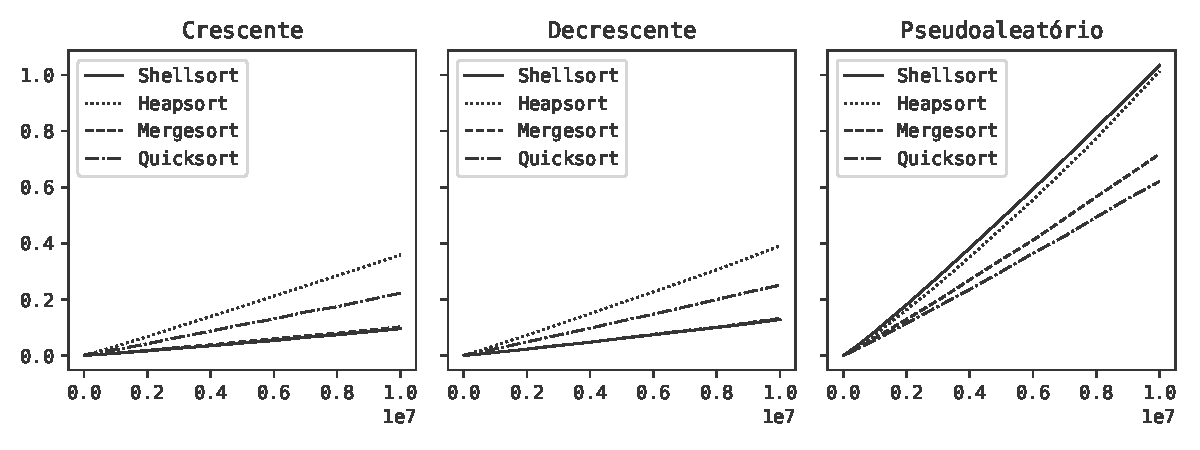
\includegraphics[scale=0.787]{figuras/pdf/superiores1e7.tempo.pdf}
\Fonte{Elaborado pelo autor}
\end{figure}

\begin{figure}[H]
\Caption{\label{fig:superiores1e8-tempo}Métodos superiores – Tamanho (até $10^8$) × Tempo.}
\centering
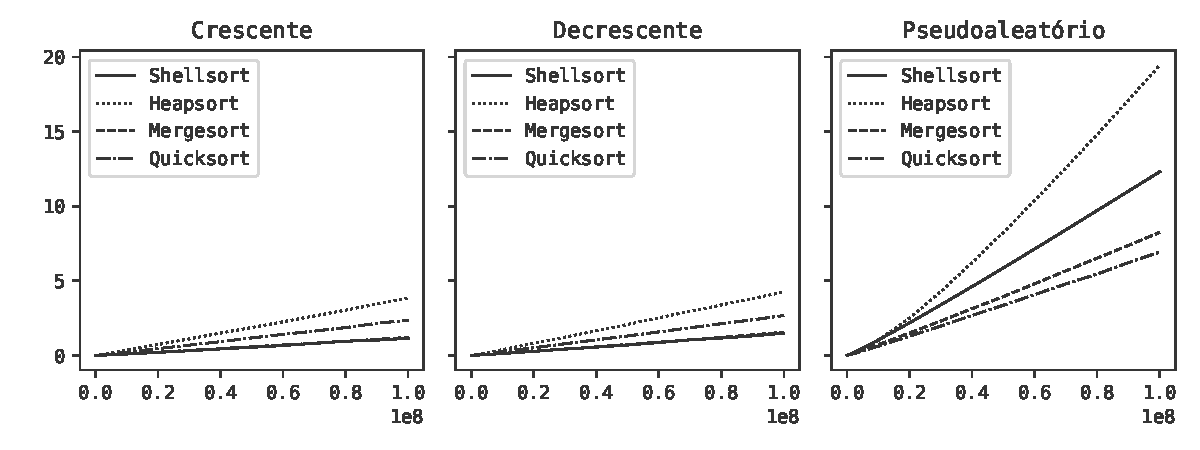
\includegraphics[scale=0.787]{figuras/pdf/superiores1e8.tempo.pdf}
\Fonte{Elaborado pelo autor}
\end{figure}

Para vetores inicialmente ordenados em ordem crescente ou decrescente, não há diferença significativa no comportamento entre a Figura \ref{fig:superiores1e7-tempo} e a Figura \ref{fig:superiores1e8-tempo}. Os algoritmos mantêm a mesma relação de desempenho entre si. Nesses casos, o Heapsort e o Quicksort apresentam seus piores cenários de execução, enquanto o Shellsort e o Mergesort se beneficiam da presença de ordem nos dados.

Já no caso geral, em ambos os gráficos, o Quicksort apresenta o melhor resultado, sendo seguido pelo Mergesort. No entanto, observa-se um comportamento atípico no Heapsort. Para vetores com tamanhos até $10^7$, como esperado pela análise teórica de complexidade, o Heapsort supera o Shellsort. Porém, para tamanhos maiores que $10^7$, o Heapsort se torna ligeiramente mais lento que todos os outros. Este fato será explicado na subseção \ref{subsec:sup-cache}.

\subsection{Comparações}
O gráfico da Figura \ref{fig:superiores.comparacoes} a seguir, exibe a relação entre o número de comparações e o tamanho do vetor para cada tipo de vetor analisado.

\begin{figure}[H]
\Caption{\label{fig:superiores.comparacoes}Métodos superiores – Tamanho × Comparações.}
\centering
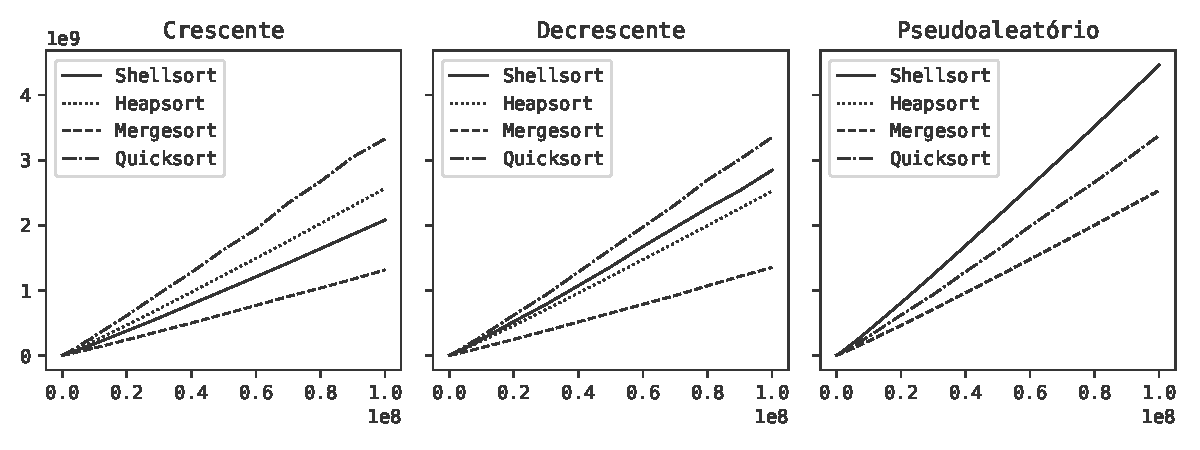
\includegraphics[scale=0.787]{figuras/pdf/superiores.comparacoes.pdf}
\Fonte{Elaborado pelo autor}
\end{figure}

Em contraste com os demais, o Quicksort e o Heapsort demonstraram estabilidade em seu desempenho. Em todos os tipos de vetor, os gráficos de ambos os algoritmos são praticamente idênticos, o que indica que a ordem inicial dos dados não os beneficia nem os prejudica. No entanto, o Heapsort executa um número ligeiramente menor de comparações do que o Quicksort.

Já o Shellsort apresentou um desempenho variável conforme o tipo de vetor. Apesar de se beneficiar quando há presença de ordem nos dados, ele foi, no caso geral, o algoritmo superior que mais executou comparações.

O Mergesort executa o menor número de comparações para todos os três tipos de vetor analisados, destacando-se em vetores já ordenados. Há uma explicação interessante para este fato: o algoritmo Mergesort só executa comparações durante o processo de Merge, e este processo se torna determinístico para vetores ordenados. Esse trecho do algoritmo é mostrado abaixo.

\lstinputlisting[language=C]{codigos/aux/merge_snippet.txt}

\subsection{Movimentações}
O gráfico da Figura \ref{fig:superiores.movimentacoes} a seguir, exibe a relação entre o número de movimentações e o tamanho do vetor para cada tipo de vetor analisado.

\begin{figure}[H]
\Caption{\label{fig:superiores.movimentacoes}Métodos superiores – Tamanho × Movimentações.}
\centering
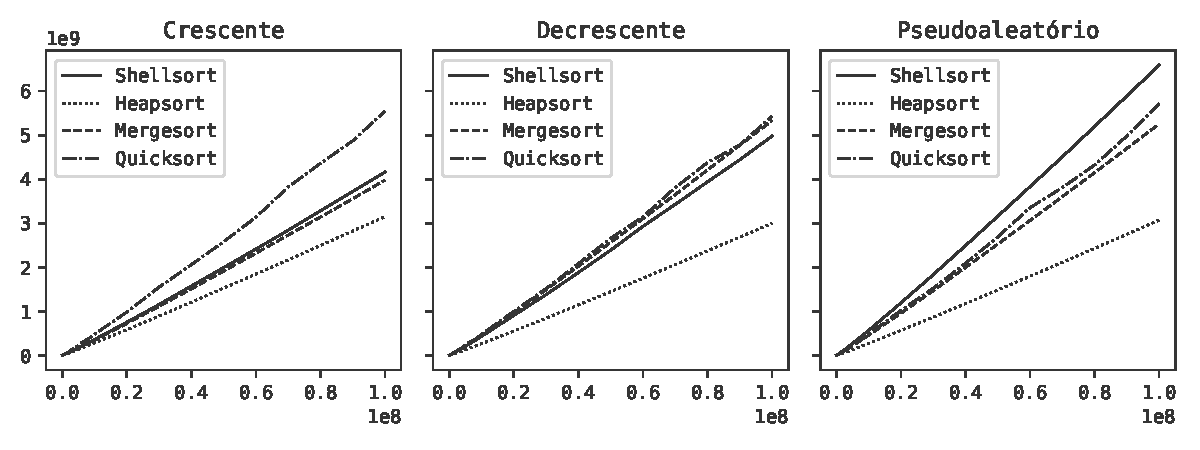
\includegraphics[scale=0.787]{figuras/pdf/superiores.movimentacoes.pdf}
\Fonte{Elaborado pelo autor}
\end{figure}

Com relação à quantidade de movimentações, o algoritmo Heapsort se destacou. Ele manteve o mesmo desempenho em todos os tipos de vetor, mas executou significativamente menos movimentações que os demais algoritmos superiores. O Quicksort também teve desempenho estável para todos os tipos de vetores, sendo ele o que mais executa movimentações para entradas já ordenadas de alguma forma. Já o Mergesort apresentou o mesmo desempenho em vetores decrescentes e no caso geral, mas executou menos movimentações para vetores crescentes, o que ocorre pelo mesmo motivo explicado na subseção anterior. De modo geral, o Shellsort é o que mais realiza a operação de movimentação de elementos do vetor de entrada.

\subsection{Eficiência de cache}\label{subsec:sup-cache}
Conforme introduzido na seção \ref{sec:arquitetura}, o processador tenta realizar a leitura e a escrita primeiramente no cache. Somente quando a informação de interesse não está presente em nenhum nível de cache, é que ele a busca na memória principal. Devido aos tamanhos de vetores utilizados neste trabalho, não é necessário mencionar a memória secundária, uma vez que toda a informação cabe na memória principal. A eficiência de cache de um algoritmo é, portanto, a taxa de sucesso na busca por elementos no cache, visto que esse acesso é muito mais rápido do que na RAM.

\subsubsection{Falhas de leitura}
O gráfico da Figura \ref{fig:superiores-DLmr} mostra a frequência em que o processador falhou ao tentar ler um dado no último nível de cache para cada algoritmo. Observe que, para vetores de tamanhos até $10^7$, e dadas as propriedades do computador utilizado nos testes, praticamente todas as leituras resultavam em sucesso. No entanto, para vetores maiores que isso, as falhas se tornaram visíveis, com o Heapsort sendo o algoritmo que mais apresentou falhas de leitura.

A explicação para a ineficiência do Heapsort reside no princípio da localidade de referência espacial, conforme detalhado na subseção \ref{subsec:localidade-referencia}. Isso ocorre porque, à medida que o algoritmo desce pelos nós do Heap, o índice de cada posição acessada é pelo menos o dobro do índice da posição acessada anteriormente. Essa característica força o carregamento de elementos novos e distantes no cache, os quais se tornam inúteis já na próxima iteração.

\begin{figure}[H]
    \Caption{\label{fig:superiores-DLmr}Métodos superiores – Falhas de leitura no último nível de cache.}
    \centering
    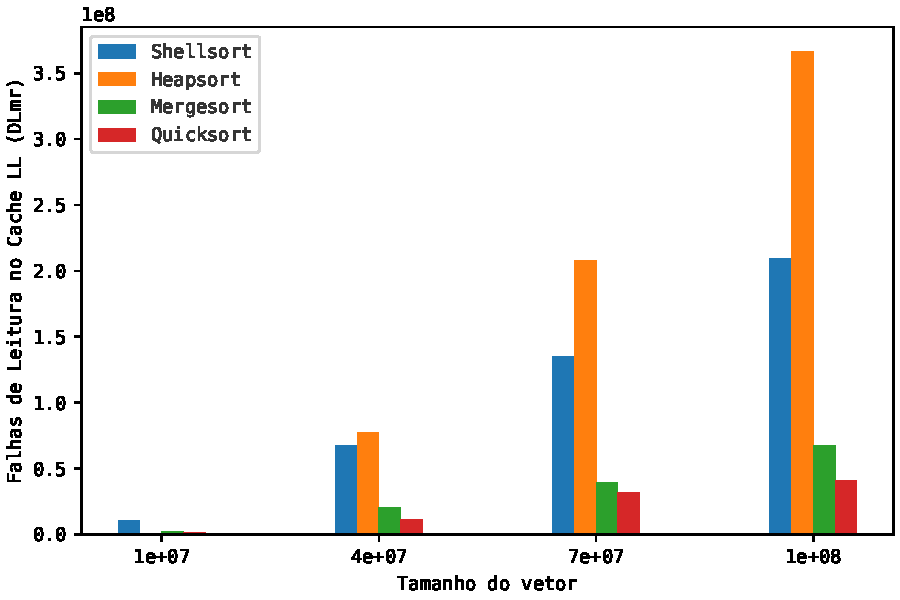
\includegraphics[scale=0.787]{figuras/pdf/superiores_DLmr.pdf}
    \Fonte{Elaborado pelo autor}
\end{figure}

\subsubsection{Falhas de escrita}
O gráfico da Figura \ref{fig:superiores-DLmw} mostra a frequência em que o processador falhou ao tentar escrever um dado no último nível de cache para cada algoritmo. Percebe-se que, mais uma vez, a quantidade de falhas é insignificante para vetores menores que $10^7$. Constata-se também que apenas o Mergesort causa falhas desse tipo. Este fato é explicado pela necessidade deste algoritmo de usar memória auxiliar.

\begin{figure}[H]
\Caption{\label{fig:superiores-DLmw}Métodos superiores – Falhas de escrita no último nível de cache.}
\centering
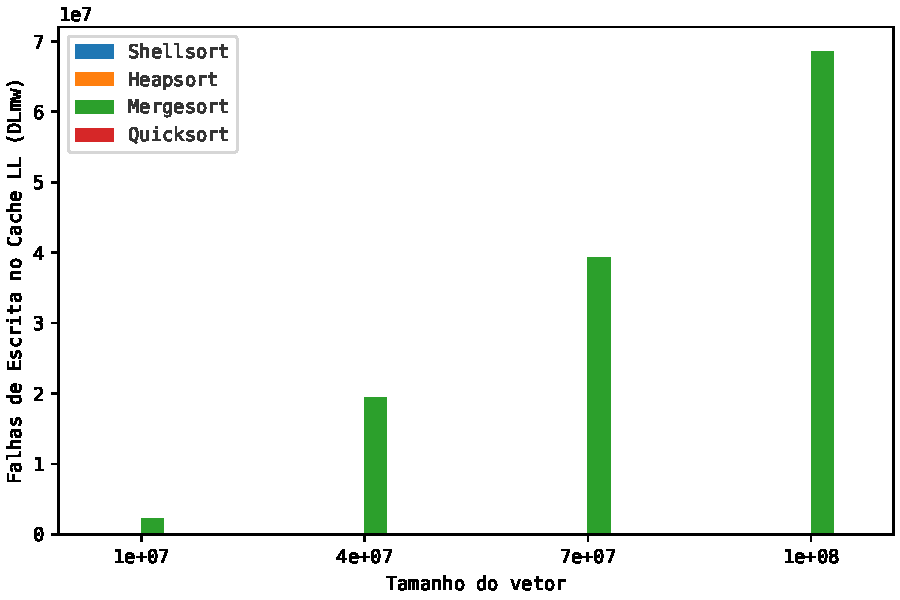
\includegraphics[scale=0.787]{figuras/pdf/superiores_DLmw.pdf}
\Fonte{Elaborado pelo autor}
\end{figure}

\subsection{Síntese dos resultados}
A Table \ref{tab:sup-classicacao} a seguir classifica os algoritmos superiores por tempo, comparações, movimentações e uso do cache, no caso geral.

\begin{table}[H]
    \centering
    \Caption{\label{tab:sup-classicacao}Métodos superiores – Classificação de desempenho por métrica}
    \begin{tabular}{ | c | l | l | l | l | l | }
        \hline
        Ranking & Tempo     & Comp.     & Movi.     & Leitura   & Escrita   \\
        \hline
        1º      & Quicksort & Mergesort & Heapsort  & Quicksort & Shellsort \\
        2º      & Mergesort & Heapsort  & Mergesort & Mergesort & Heapsort  \\
        3º      & Shellsort & Quicksort & Quicksort & Shellsort & Quicksort \\
        4º      & Heapsort  & Shellsort & Shellsort & Heapsort  & Mergesort \\
        \hline
    \end{tabular}
\end{table}

O Quicksort, apesar de não ser o algoritmo que realiza menos comparações ou movimentações, é o mais eficiente em termos de cache. Essa eficiência o estabelece como o melhor algoritmo superior para a principal métrica, o tempo. Já o Shellsort é o que mais executa comparações e movimentações, mas ainda assim acaba sendo mais rápido que o Heapsort, também devido à sua eficiência de cache. Por fim, o Mergesort é quase tão bom quanto o Quicksort, sendo penalizado pelo uso de memória extra.

\section{Quicksort e métodos híbridos}
Os algoritmos de ordenação mais utilizados na prática são híbridos, baseados no Quicksort. Tais algoritmos se beneficiam dos pontos positivos do Quicksort ao mesmo tempo em que tentam diminuir o número de movimentações realizadas e evitar o pior caso.

No capítulo anterior, foram apresentados dois algoritmos desse tipo: o QuicksortI, que utiliza a Inserção para finalizar a ordenação, reduzindo o número de movimentações; e o Introsort, algoritmo utilizado na biblioteca padrão da linguagem de programação C\raisebox{0.4ex}{\text{\tiny{++}}}.

O Introsort também utiliza a Inserção para finalizar a ordenação, mas usa o Heapsort quando a árvore de recursão atinge altura igual a $2\log n$, contornando assim os casos em que o Quicksort tende ao pior cenário. O gráfico da Figura \ref{fig:hibridos} a seguir mostra os resultados de tempo e movimentações do Quicksort em comparação com o QuicksortI e o Introsort. Os resultados com relação ao número de comparações foram equivalentes e, por isso, não serão mostrados.

\begin{figure}[H]
\Caption{\label{fig:hibridos}Métodos híbridos – Tempo e movimentações.}
\centering
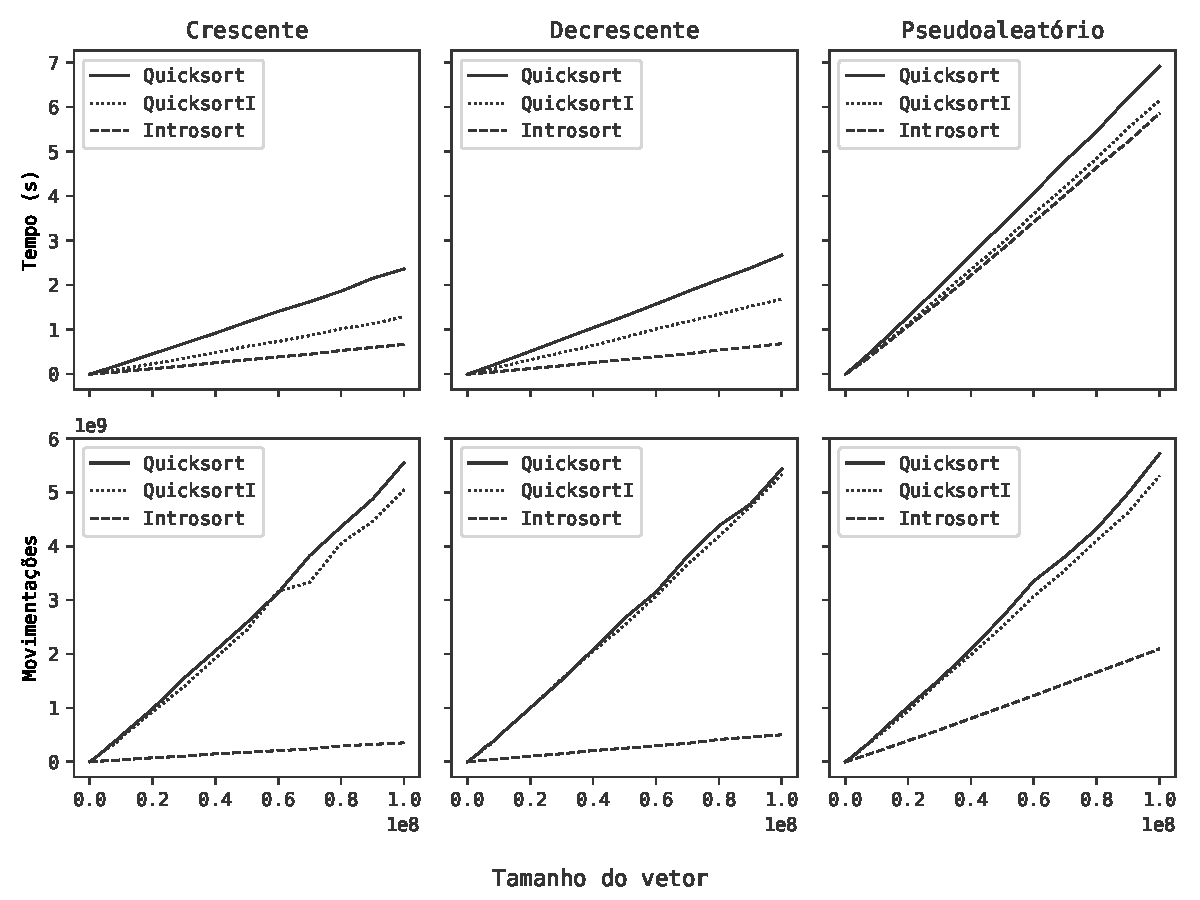
\includegraphics[scale=0.787]{figuras/pdf/hibridos.pdf}
\Fonte{Elaborado pelo autor}
\end{figure}

\section{Métodos lineares}
A subseção \ref{subsec:cota-inferior} mostrou que a cota inferior para algoritmos baseados em comparação é $\Omega(n\log_2n)$. Isso significa que, para um algoritmo ser linear, ele não pode se basear em comparação. Além disso, os algoritmos lineares de ordenação apresentados neste trabalho só são lineares para entradas que obedecem a certas propriedades. Por exemplo, o Countingsort assume que os elementos da entrada podem ser indexados e que a diferença entre o maior e o menor elemento é limitada por uma constante suficientemente pequena para caber na memória. Já o Bucketsort requer que os elementos estejam uniformemente distribuídos em um intervalo. Por fim, o Radixsort assume que o algoritmo auxiliar é estável e linear e que cada elemento da entrada pode ser decomposto em dígitos pertencentes a um conjunto limitado e ordenável. Todos esses pré-requisitos foram levados em consideração nos testes, e todos os vetores foram gerados de modo a manter a característica linear de cada algoritmo.

\begin{figure}[H]
\Caption{\label{fig:lineares}Métodos lineares – Tempo e movimentações.}
\centering
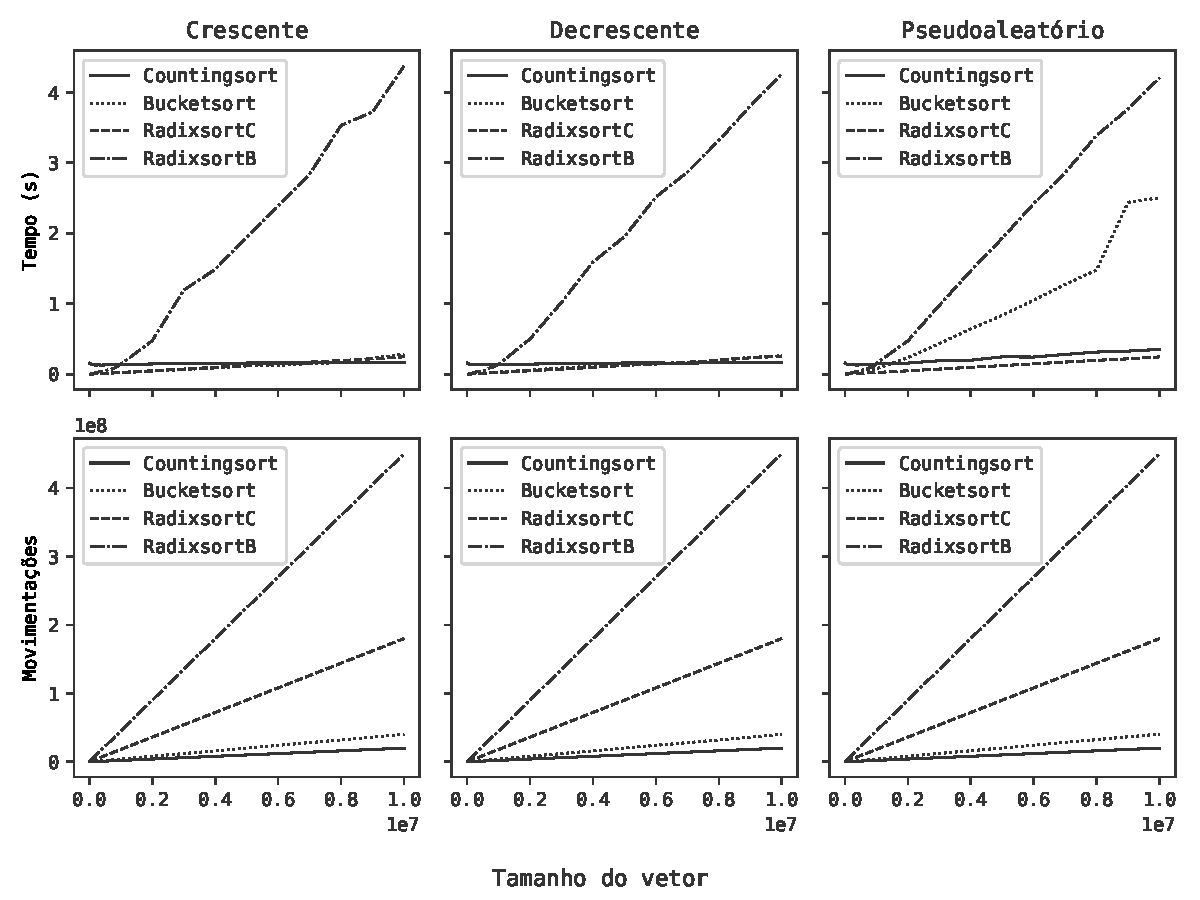
\includegraphics[scale=0.787]{figuras/pdf/lineares.pdf}
\Fonte{Elaborado pelo autor}
\end{figure}

O primeiro ponto a se observar é que cada algoritmo apresenta consistência no número de movimentações. Isso ocorre porque cada um deles, independentemente do tipo de vetor, move os dados para a memória auxiliar e, em seguida, os traz de volta para o vetor de entrada, de modo a garantir a ordenação.

No entanto, ambas as versões do Radixsort — tanto a que usa o Countingsort como sub-rotina quanto a que usa o Bucketsort — executam mais movimentações. Isso se deve ao fato de que elas têm que realizar a movimentação para a memória auxiliar nove vezes, pois essa é a quantidade máxima de dígitos que cada número da entrada pode ter.

Por fim, observamos outros dois comportamentos que o gráfico não explica. O primeiro é que o RadixsortC foi mais rápido que o Countingsort, mesmo executando mais movimentações. Isso ocorre porque o RadixsortC utiliza menos memória que o Countingsort, uma vez que o vetor que armazenaria a frequência de cada elemento da entrada no Countingsort aloca $10^8$ posições, enquanto que no RadixsortC aloca apenas $10$.

O segundo é que o Bucketsort se tornou consideravelmente mais lento para vetores gerados de forma pseudoaleatória. Isso ocorre porque, mesmo que os elementos tendam a ser igualmente prováveis na geração do vetor, não é o que ocorre exatamente na prática. Para vetores crescentes ou decrescentes, devido à forma como os elementos foram escolhidos na geração dos vetores, cada bucket recebeu entre $0$ e $2$ elementos, o que não sobrecarrega a versão do Insercao utilizada. Já para vetores gerados de forma pseudoaleatória, os buckets tiveram entre $0$ e $9$ elementos, como mostra a Figura \ref{fig:frequencia-buckets}. Esse desequilíbrio fez com que o Insercao precisasse executar mais operações na lista ligada utilizada, o que tornou o algoritmo mais lento nesses casos.

\begin{figure}[H]
\Caption{\label{fig:frequencia-buckets}Bucketsort – Frequência de tamanho de bucket ($10^7$ elementos)}
\centering
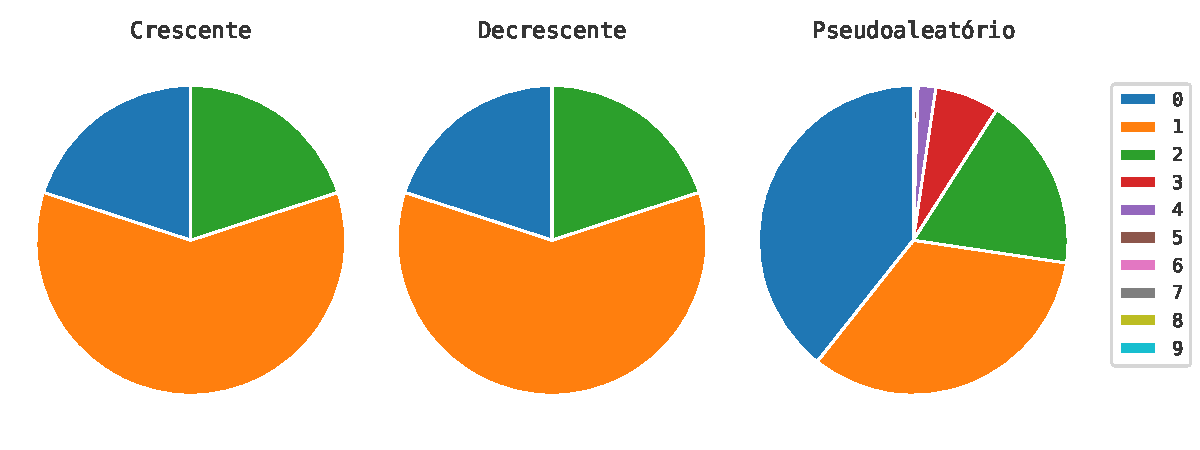
\includegraphics[scale=0.787]{figuras/pdf/frequencia_buckets.pdf}
\Fonte{Elaborado pelo autor}
\end{figure}

\chapter{Conclusão}\label{cap:conclusao}
- Falar sobre o que FOI feito neste trabalho


% Elementos pós-textuais
\bibliography{elementos-pos-textuais/referencias}

\end{document}
